\vspace{0.25em}

% \x changed to XXX

\renewcommand{\thefootnote}{\arabic{footnote}}
\setcounter{footnote}{0}

\chapter*{Introduction}

\section{History of the STEDT project}

The great Sino-Tibetan language family, comprising both Chinese and Tibeto-Burman (TB),\footnote{Some scholars, especially in China, consider Sino-Tibetan to include the Tai-Kadai (TK) and Hmong-Mien (HM) (=Mi\'ao-Y\'ao) language families as well.  While there is definitely a striking typological similarity among Chinese, TK, and HM, this is undoubtedly due to prolonged ancient contact rather than genetic relationship.  See \citealt{PB-ATLC} (\textit{Austro-Thai Language and Culture, with a glossary of roots}).} is comparable in time-depth and internal diversity to Indo-European, and equally important in the context of world civilization. The overwhelming cultural and numerical predominance of Chinese is counterbalanced by the sheer number of languages (some 250–300) in the rest of the family.

After the existence of Tibeto-Burman family was posited in the mid-19th century, British scholars, missionaries, and colonial administrators in India and Burma began to study some of the dozens of little-known “tribal” languages of the region that seemed to be genetically related to the two major literary languages, Tibetan and Burmese. This early work was collected in the monumental \textit{Linguistic Survey of India} (\citealt{LSI}), three sections of which (Vol.~III, Parts 1, 2, 3) are devoted to wordlists and brief texts from TB languages.

Further significant progress in TB studies had to wait until the late 1930’s, when the eccentric amateur comparativist Robert Shafer headed a Depression-era project called “Sino-Tibetan Linguistics”, sponsored by the eminent anthropologist A.L.\ Kroeber of U.C.\ Berkeley.\footnote{For a readable and humorous account of this project, see Benedict 1975b.} With admirable thoroughness, the project staff assembled all the lexical material then available on TB languages, enabling Shafer to venture a detailed subgrouping of the family at different taxonomic levels, called (from higher to lower) divisions, sections, branches, units, languages, and dialects. This work was finally published piecemeal in a two-volume, five-part opus called Introduction to Sino-Tibetan (1966–67; 1974).

Shafer’s junior collaborator Paul K.\ Benedict based his own work on the same body of material as Shafer, but achieved much more usable results. In an unpublished manuscript entitled Sino-Tibetan: a Conspectus (ca.\ 1942–43; henceforth \textit{STC}), Benedict adopted a more modest approach to supergrouping and subgrouping than Shafer, stressing that many TB languages had so far resisted precise classification. While Shafer had included Tai in Sino-Tibetan, Benedict (1942) banished it from the family altogether, relating Tai instead to Austronesian.\footnote{To this putative megalolinguistic grouping, later to include Hmong-Mien and Japanese as well as Tai-Kadai and Austronesian, Benedict gave the name “Austro-T(h)ai” (see \citealt{PB-ATLC,PB-ATJ}).} Shafer’s pioneering work, valuable as it was, suffered from his mistrust of phonemics, with a consequent proliferation of pseudo-precise and arcane phonetic symbols. Benedict’s structural insight, his flair for isolating that which is crucial from masses of data  enabled him to formulate sound correspondences with greater precision, and to distinguish between regular and exceptional phonological developments.

The publication of a revised and heavily annotated version of \textit{STC} in 1972, with J.\ Matisoff as contributing editor, laid the foundations for modern Sino-Tibetan historical/\allowbreak{}comparative linguistics. In this recension, nearly 700 Proto-Tibeto-Burman (PTB) roots were reconstructed (494 of them in numbered cognate sets, with about 200 more scattered throughout the text and footnotes), as well as some 325 comparisons of PTB roots with Old Chinese etyma, largely as reconstructed by \citet{GSR}. While Benedict focussed principally on five key, phonologically conservative TB languages (Tibetan, Burmese, Lushai [=Mizo], Kachin [=Jingpho], Garo), he also used data from more than 100 others, judiciously making allowances for inadequacies of transcription where necessary.\footnote{In a recently published work, \citet{PS-STL} follow Benedict’ s example in their choice of key TB languages, basing their Sino-Tibetan reconstructions on Written Tibetan, Written Burmese, Lushai, Jingpho, and Chinese, all of which are treated as if they belonged on the same taxonomic level. See the discussion in \citet[ch.\ 3]{ZH-OCST98}.} How well has \textit{STC} stood the test of time? The short answer is: remarkably well. The work has been reviewed about 15 times, almost always in a highly favorable tone,\footnote{A notable exception is the intemperate review by \citet{RAM-STIC}, which bitterly criticizes the fact that the notes added in 1972 sometimes modify points made in the original text (ca.\ 1942). See the defense of \textit{STC} against Miller’s attack by\citet{JAM-BST}.} and has been translated into Chinese.\footnote{See \citealt{HZYG}.} In fact nearly all 700 of the TB cognate sets in \textit{STC} have been shown to be perfectly valid, though many of the reconstructions have had to be changed slightly in the light of new data, and in a couple of cases etyma which had been reconstructed separately have been shown to be variant forms (“allofams”) of the same word-family.\footnote{e.g.\ \textbf{*dyam} \& \textbf{*tyam} [\textit{STC} $\#$226] ‘full; fill’ and \textbf{*dyam} [\textit{STC} $\#$227] ‘straight’ ; see \citet{JAM-USAI}.}

Despite its brilliance, however, the {\it Conspectus} is notoriously difficult to use, largely due to its complex apparatus of footnotes, which often (especially in the Chinese section) occupy more of the page than the text itself. These notes include Benedict’s original ones from the 1940’s, as well as those he and I added before publication in 1972. Some 200 valid etymologies are squirreled away in these convoluted notes, but they also contain a number of errors, unsubstantiated speculations, and over-complications.

Benedict himself realized the limitations of the data he had to work with, and never intended \textit{STC} to be more than an overview or “conspectus” of its vast subject. Neither did he structure it as a practical handbook which systematically tabulated the sound correspondences among the major languages of the family at all canonical points of the syllable. (Such information is certainly extractable from the terse but labyrinthine pages of \textit{STC}, but at the cost of considerable labor.) Towards the end of his life, which ended tragically in a car accident on July 21, 1997, Benedict does seem to have felt the need to embark on such a systematic project, although it never actually got off the ground.

After the publication of the {\it Conspectus}, further progress in intra-TB and TB/Chinese comparison seemed to depend on multiplying the number of reliably reconstructed etyma, as well as systematizing and refining the methodological underpinnings of the reconstructions. In the mid-1970’s, when I was attempting to apply the principles of glottochronology in order to subgroup the TB family, the very first item of “basic vocabulary” that I looked at happened to be ‘belly / stomach’. Much to my initial dismay, I quickly found that it was futile to use a simple wordlist to try to subgroup a family as complex and ramified as TB. In fact it was impossible even to deal in isolation with a single point in semantic space; etyma with the meaning ‘belly’ or ‘stomach’ spilled over into concepts like ‘cave / hole’, ‘swelling’, ‘calf of leg’, ‘liver’, ‘guts’, etc. I became preoccupied with notions of semantic variability, semantic fields, and the field of bodypart nomenclature in particular. At the same time I could not help noticing the morphophonemic variations displayed by almost every etymon previously or newly reconstructed. Instead of guiltily sweeping these variational phenomena under the rug, I began to revel in them. In {\it Variational Semantics in Tibeto-Burman} \citep{VSTB} I set out to establish an explicit methodology for handling phonosemantic variation in word families, introducing the notion of “allofams” and a notation for diagramming patterns of semantic association (“metastatic flowcharts”). In those pre-computer days, I naturally had to assemble my data by hand, copying out bodypart words from dictionaries and sorting them into synonym sets on filecards, then grouping them into putative cognate sets. The older sources used by Shafer and Benedict were supplemented by an ever-increasing volume of new material in the 1970’s and 1980’s, much of it from post-Cultural Revolution China, but also from India, Nepal, and Thailand. It eventually became apparent that the job of digesting these massive amounts of new and old data would be vastly facilitated by the use of computers. The hitch was my own ignorance of computer technology beyond the level of simple word-processing. Fortunately I somehow got the idea of applying to federal granting agencies for a longterm project to create a computerized etymological dictionary of Tibeto-Burman / Sino-Tibetan based on semantic principles, i.e.\ an etymological thesaurus.\footnote{The shining example of an etymological thesaurus in the field of Indo-European is Carl Darling Buck’s {\it A Dictionary of Selected Synonyms in the Principal Indo-European Languages} (1949).} In 1987, the Sino-Tibetan Etymological Dictionary and Thesaurus Project (STEDT) got under way, funded jointly by the National Science Foundation and the National Endowment for the Humanities. Thanks to the efforts of a succession of computer-savvy graduate students (see the {\it Acknowledgments}), a massive lexical database of forms from over 250 TB languages and dialects has been created, mostly of bodypart terminology at first, but then extending to all the other areas of the lexicon. It has been a race between the vertiginous progress of computer technology (when we started in the Pleistocene, 1987, we were using Mac Pluses!) and our ever-expanding needs for disk capacity, memory, and operating speed. The hardwon experience gained at the STEDT project has inspired similar lexical database projects in the U.S.\ and abroad.

\section{Original Plan of STEDT}

It was originally planned to publish the {\it Sino-Tibetan Etymological Dictionary and Thesaurus} as a series of printed volumes, each containing full details on all the etymologies in a given semantic area, starting with bodyparts and then proceeding to animal names, natural objects, verbs of motion, and all the rest of the lexicon:

\begin{quote}
{\footnotesize
Volume I: \textit{Body Parts}\nopagebreak[4]\\
Volume II: \textit{Animals}\\
Volume III: \textit{Natural Objects, Plants, Foods }\\
Volume IV: \textit{Kinship Terms, Ethnonyms, Social Roles}\\
Volume V: \textit{Culture, Artifacts, Religion}\\
Volume VI: \textit{Verbs of Motion, of Manipulation, and of Production}\\
Volume VII: \textit{Adjectival Verbs}\\
Volume VIII: \textit{Abstract Nouns and Verbs, Psychological Verbs, Verbs of Utterance }\\
Volume IX: \textit{Shape, Size, Color, Measure, Number, Time, Space}\\
Volume X: \textit{Grammatical words}\\
}
\end{quote}

 The sheer amount of the etymologizable data soon made it clear that this was unrealistic, and that each projected volume of STEDT would have to be split up into smaller units or “fascicles”, e.g.\ in the case of \textit{Body Parts} into ten subdivisions, as follows:

\begin{quote}
{\footnotesize
1. \textit{Body (general)}\\
2. \textit{Head and Face}\\
3. \textit{Mouth and Throat}\\
4. \textit{Torso}\\
5. \textit{Limbs, Joints, and Body Measures}\\
6. \textit{Diffuse Organs}\\
7. \textit{Internal Organs}\\
8. \textit{Secretions and Somatophonics}\footnote{By ‘somatophonics’ I mean sneezes,
belches, farts, and the like.}\\
9. \textit{Reproductive System}\\
}
\end{quote}

Every subpart and sub-subpart of the lexicon expanded and bloomed into a major project.

Concentrated on NBP’s --- TBRS was fascicle 9 of Vol.~I.

I decided to start with the reproductive system, not only because of its prurient interest but also because it seemed like the point of departure for all things. Accordingly a printed manuscript of some 480 pages was produced in 1997–98, called Sino-Tibetan Etymological Dictionary and Thesaurus, Volume I: Bodyparts, Fascicle 1: The Reproductive System, containing 286 pages of forms assembled into 174 cognate sets, divided into nine chapters: (1) Egg, (2) Birth, (3) Navel, (4) Breast, (5) Vagina, (6) Womb, (7) Penis, (8) Copulate, (9) Body Fluids. As part of the front matter, I put together a 60 page essay on the initial consonants and consonant clusters of Proto-Tibeto-Burman.

As it turned out, perhaps fortunately, that introductory essay soon took on a teratoid life of its own, and became an example of what one might call in Proto-Tibeto-Burman 
\begin{quote}
\begin{center}
\begin{tabular}{l l l l l}
\textbf{*kʷəy} & \textbf{lətak} & \textbf{rəmay} & \textbf{gəyaːp} & \textbf{way}\\
dog & ACC & tail & wag & COP/NOM
\end{tabular}
\end{center}
\end{quote}
or “the tail wagging the dog”.\footnote{The presence of the accusative particle \textbf{*lətak} is motivated by the semantic anomalousness of this phrase, which has also caused the fronting of the object \textbf{*kʷəy} ‘dog’ to initial position.} Was I not responsible for dealing with the whole proto-syllable, not just the initial consonants? I delayed publication of the “Reproductive Fascicle” until I could get the whole job done.\footnote{It was later published
as \citealt{TBRS}.}
Eventually, the “introductory essay”, then entitled \textit{System and Philosophy of Tibeto-Burman Reconstruction}, grew to become \textit{Handbook of Proto-Tibeto-Burman} (henceforth \textit{HPTB}).


The phonological approach of HPTB is complementary to the main thrust of the STEDT project, which is semantically organized.

\section{The ST/TB Family in it Areal Context}

\subsection{Typological diversity of TB: Indosphere and Sinosphere}

The TB family, which extends over a huge geographic range, is characterized by great typological diversity, comprising languages that range from the highly tonal, monosyllabic, analytic type with practically no affixational morphology (e.g.\ Loloish), to marginally tonal or atonal languages with complex systems of verbal agreement morphology (e.g.\ the Kiranti group of E.\ Nepal). While most TB languages are verb-final, the Karenic and Baic branches are SVO, like Chinese.
 
This diversity is partly to be explained in terms of areal influence from Chinese on the one hand, and Indo-Aryan languages on the other. It is convenient to refer to the Chinese and Indian spheres of cultural influence as the “Sinosphere” and the “Indosphere”.\footnote{See \citealt{JAM-OM} (“On megalocomparison.”)} Some languages and cultures are firmly in one or the other: e.g.\ the Munda and Khasi branches of Austroasiatic, the TB languages of Nepal, and much of the Kamarupan branch of TB (notably Meithei = Manipuri) are Indospheric; while the Hmong-Mien family, the Kam-Sui branch of Kadai, the Loloish branch of TB, and Vietnamese (Mon-Khmer) are Sinospheric. Others (e.g.\ Thai and Tibetan) have been influenced by both Chinese and Indian culture at different historical periods. Still other linguistic communities are so remote geographically that they have escaped significant influence from either cultural tradition (e.g.\ the Aslian branch of Mon-Khmer in Malaya, or the Nicobarese branch of Mon-Khmer in the Nicobar Islands of the Indian Ocean).

Elements of Indian culture, especially ideas of kingship, religions (Hinduism/Brahminism, Buddhism), and {\it devan\=agar\={\i}} writing systems, began to penetrate both insular and peninsular Southeast Asia about 2000 years ago. Indic writing systems were adopted first by Austronesians (Javanese and Cham) and Austroasiatics (Khmer and Mon), then by Tai (Siamese and Lao) and Tibeto-Burmans (Pyu, Burmese, and Karen). The learned components of the vocabularies of Khmer, Mon, Burmese, and Thai/Lao consist of words of Pali/Sanskrit origin. Indian influence also spread north to the Himalayan region. Tibetan has used {\it devan\=agar\={\i}} writing since A.D.\ 600, but has preferred to calque new religious and technical vocabulary from native morphemes rather than borrowing Indic ones.

What is now China south of the Yangtze did not have a considerable Han Chinese population until the beginning of the current era (Ramsey 1987, Norman 1988). In early times the scattered Chinese communities of the region must have been on a numerical and cultural par with the coterritorial non-Chinese populations, with borrowing of material culture and vocabulary proceeding in all directions \citep{PB-ATLC,MeiNorman1976,Sagart1990}. As late as the end of the first millennium A.D., non-Chinese states flourished on the periphery of the Middle Kingdom (Nanchao and Bai in Yunnan, Xixia (Tangut) in the Gansu/Qinghai/Tibet border regions, Lolo (Yi) chieftaincies in Sichuan. The Mongol Yuan dynasty finally consolidated Chinese power south of the Yangtze in the 13th century. Tibet also fell under Mongol influence then, but did not come under complete Chinese control until the 18th century.

Whatever their genetic affiliations, the languages of the East and SE Asian area have undergone massive convergence in all areas of their structure  phonological, grammatical, and semantic.\footnote{An excellent recent study of such phenomena is Thomason and Kaufman 1988.}  Hundreds of words have crossed over genetic boundaries in the course of millennia of intense language contact, so that it is often exceedingly difficult to distinguish ancient loans from genuine cognates.

\subsection{Scope and subgrouping of the TB family}

The exact number of TB languages is impossible to determine, not only because of the elusiveness of the distinction between “languages” and “dialects,” and the fact that a number of languages remain to be discovered and/or described, but especially because of the profusion and confusion of different names for the same language.\footnote{See JAM 1986a, and STEDT Monograph II (JAM 1996a).} At the present state of our knowledge we can estimate that the Tibeto-Burman family contains approximately 250 languages, which may be broken down into population categories as indicated in Table 1.\footnote{Based on \citealt{G-ELW}}

[table 1]

According to official estimates, there are nine Tibeto-Burman languages with over a million speakers: Burmese, Tibetan, Bai, Yi (= Lolo), Karen, Meithei (= Manipuri), Tujia, Hani, Jingpho. This is quite misleading, however, since ethnic identity and linguistic competence do not always coincide: of the [XXX] people who identify themselves as Tujia, only about 50,000 can actively use the Tujia language, the rest having shifted to Chinese. Designations like {\it Yi} and {\it Karen} actually apply to large numbers of related but often not mutually intelligible “dialects”, which might as well be called separate languages. At the bottom of the scale are some 125 languages with fewer than 10,000 speakers, many of which are highly endangered,\footnote{See \citealt{Matisoff1991b}.} to the point where children are no longer learning to speak them.

Although much of the geographical area covered by TB languages\footnote{Very approximately, the distribution of TB languages by country is as follows: India 107, Burma 75, Nepal 69, China 50, Thailand 16, Bangladesh 16, Bhutan 9, Laos 8, Vietnam 8, Pakistan 1.} has been chronically inaccessible to fieldwork by scholars from outside, there has been an explosion of data in the past 25 years, especially from China\footnote{Among the most valuable of these new sources are Sun Hongkai, Xu Jufang {\it et al.} \citep{ZMYYC}, containing 1004 synonym sets in 52 languages and dialects; and Dai Qingxia and Huang Bufan \citep{TBL}, with 1822 synonym sets in 50 languages and dialects.} and Nepal, but also increasingy from India and Burma.

\subsection{Evolving notions of ST/TB subgrouping}

Millennia of language contact due to migrations, intermarriage, and warfare have presented us what I
have described as ‘an interlocking network of fuzzy-edged clots of languages,
emitting waves of mutual influence from their various nuclear ganglia. A mess,
in other words.’\footnote{\citealt{JAM-VSTB} (\textit{VSTB}), p.~2.}  While subgrouping such
a recalcitrant family is difficult, there is certainly no need to go so far as
van Driem by denying that TB subgroups exist at all, or by claiming that even if
they do exist, there are so many of them that there is no point in talking about
them!\footnote{See his review (2003) of \citealt{STL},
\textit{The Sino-Tibetan Languages}.}


In the published version of \textit{STC} (1972),
P.K.\ Benedict wisely refrained from offering a pseudo-precise family-tree model of
the higher-order taxonomic relationships in TB, presenting instead a schematic
chart where Kachin (=~Jingpho) was conceived as the center of geographical and
linguistic diversity in the family. See Fig.~1.

\begin{figure}[ht]
% \XeTeXpdffile "../../pdf/intro231.pdf" 
\resizebox{\columnwidth}{!}{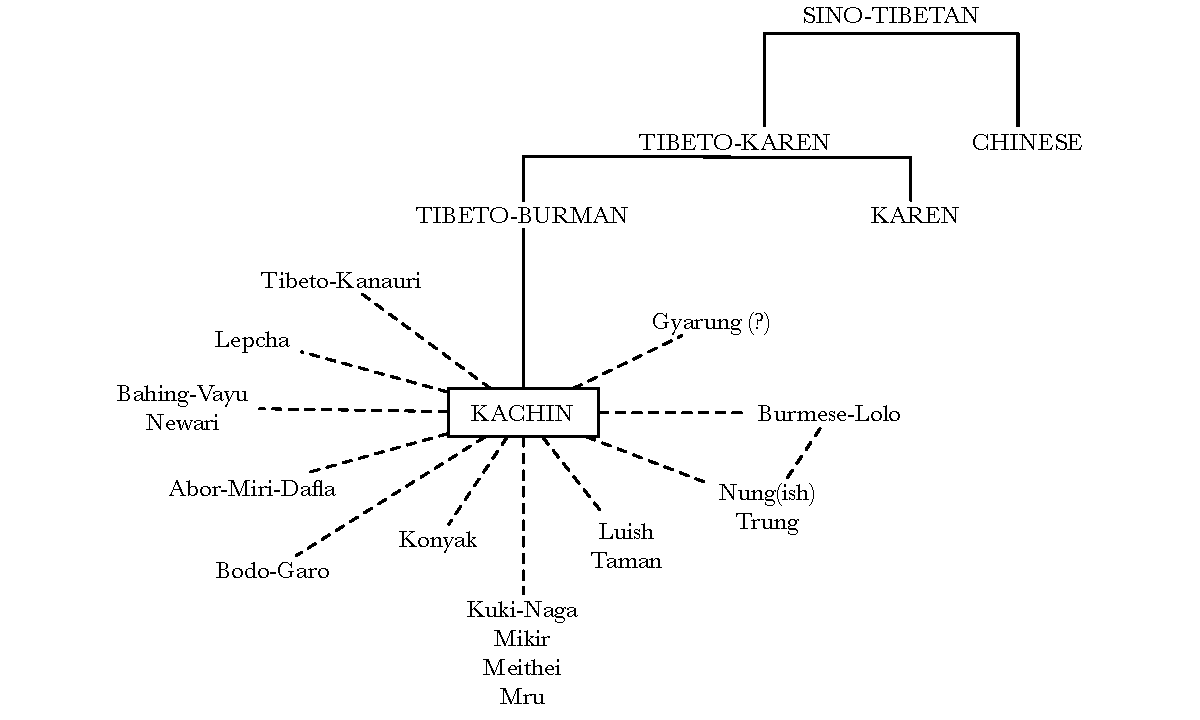
\includegraphics{../../pdf/intro231.pdf}}
\begin{center}
\textit{Figure 1.~Schematic Chart of Sino-Tibetan Languages}\footnotemark
\end{center}
\end{figure}
\footnotetext{Reproduced from \textit{STC}, p.~6;
\textit{VSTB}, p.~3; \textit{HPTB}, p.~4.}

A simpler scheme has been used heuristically at STEDT until very recently (see HPTB:5 and TBRS:xxix), as shown in  See Fig.~2. It differs from \textit{STC} in several respects:

\begin{figure}[ht]
% \XeTeXpdffile "../../pdf/intro232.pdf"
\resizebox{\columnwidth}{!}{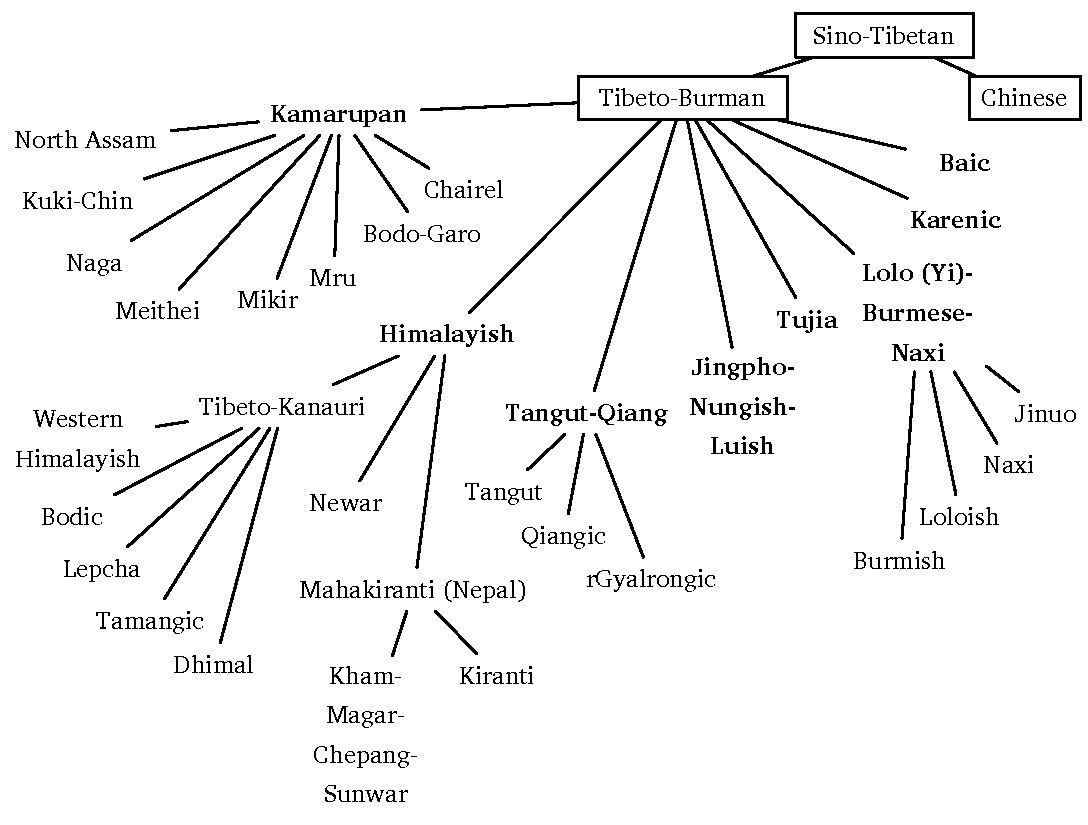
\includegraphics{../../pdf/intro232.pdf}}
\begin{center}
\textit{Figure 2.~Simplified STEDT Family Tree of ST Languages}
\end{center}
\end{figure}

\begin{itemize}
\item Karenic is no longer regarded as having a special status, but is now
considered to be a subgroup of TB proper.
\item Baic, hardly mentioned (under the name ‘Minchia’) in \textit{STC}, but later
hypothesized by Benedict to belong with Chinese in the ‘Sinitic’ branch of 
Sino-Tibetan, is now also treated as just another subgroup of TB, though one
under particularly heavy Chinese contact influence. Both Karenic and Baic have
SVO word order, unlike the rest of the TB family.
\item The highly ramified Kuki-Chin and Naga groups were provisionally
amalgamated with Bodo-Garo (=Barish) and Abor-Miri-Dafla (=Mirish) into a
supergroup called by the purely geographical name of \textit{Kamarupan}, from the old
Sanskrit name for Assam.
\item The important Tangut-Qiang languages (deemed to include rGyalrong
[=Gyarung =Jiarong] and the extinct Xixia [=Tangut]) were hardly known to Western
scholars at the time \textit{STC} was written (ca.~1942–3) or published (1972). It seems
doubtful that a special relationship exists between Qiangic and Jingpho, or
between Qiangic and Lolo-Burmese, as some Chinese scholars maintain.\footnote{A
supergroup called ‘Rung’ was proposed by \citet{GT-Rung}, into which he placed,
among others, some Qiangic languages, Nungish, and Lepcha. This grouping was
based partly on shared ‘proto-morphosyntax’, and partly on nomenclature,
including the \textit{-rong} of \textit{rGyalrong},
the Nungish language \textit{Rawang}, and the Lepcha autonym \textit{Rong}.}
\item The Nungish and Luish languages were grouped with Jingpho (=Kachin). Jingpho
is also recognized to have a special contact relationship with the Northern Naga
(=Konyak) group.\footnote{The \textit{Linguistic Survey of India}
\citep{LSI} recognized a ‘Bodo-Naga-Kachin’ group,
an idea revived by \citet{RB-Sal}, whose ‘Sal’ supergroup comprises Bodo-Garo (Barish), Northern Naga
(Konyak), and Jingpho (=Kachin). Burling’s name for this grouping is derived
from the etymon \textbf{*sal} ‘sun’ (ult.\ < PTB \textbf{*tsyar} ‘sunshine’), one of a number of
roots which is attested chiefly in these languages. See \textit{HPTB}:393–4.}
\item The somewhat idiosyncratic Mikir, Meithei (=Manipuri), and Mru languages are
included under Kamarupan.
\item The Himalayish (=Himalayan) group is considered to include Bodic (i.e.\
\mbox{Tibetanoid}) languages, as well as Kanauri-Manchad, Tamang-Gurung-Thakali,
Kiranti (=Rai), Lepcha, and Newar. It remains to be seen whether this is anything more than a geographic grouping.
\item The relatively well-studied Lolo-Burmese group (= \textit{STC}’s ‘Burmese-Lolo’) is
deemed to include the aberrant slightly Jinuo language of Xishuangbanna,
Yunnan.\footnote{Chinese scholars have further divided the Loloish languages of
China into six nuclei, although no attempt is made in this volume to distinguish
them. In Matisoff 2007b I examined Loloish tonal developments
and the fate of the PLB rhyme \textbf{*-a} in terms of this six-way grouping, with
inconclusive results.}  The Naxi/Moso language is quite close to LB, but stands
somewhat outside the core of the family.\footnote{I have grouped Naxi with
Lolo-Burmese proper in a supergroup called ‘Burmo-Naxi-Lolo’ (Matisoff 1991c).
On the basis of some shared tonal developments, I have also entertained the idea
of a special relationship between Lolo-Burmese and Jingpho, to which I assigned
the jocular designation \textit{Jiburish} (<~\textbf{Ji-}(ngpho)
+ \textbf{-bur}(mish) + (Lolo)\textbf{ish}). See \citealt{JAM-TJLB,JAM-JR}.}
\item The rather mysterious Tujia language of Hunan and Hubei (not mentioned in \textit{STC}) has so
far not been assigned to a subgroup.
\end{itemize}

My most up-to-date reconsideration of TB subgrouping has been motivated by very recent research on the Luish languages \citep{Huziwara2008,Huziwara2012,Sangdong2013}, as well as on Jingpho dialects \citep{Kurabe2013}. It now seems clear that Jingpho’s closest relatives are the formerly obscure languages of the Luish\footnote{This group needs to be renamed (I suggest Asakian), since “Luish” is a pejorative exonym. See below 2.3.} group, with the Northern Naga group also fairly close, and the Bodo-Garo group more distantly related. On the other hand, Nungish (once believed to be especially close to Jingpho) now seems to constitute an independent subgroup, so that the many lexical similarities it shows with Jingpho are due to contact rather than to any particularly close genetic relationship.\footnote{If anything, Nungish now seems to be closer to LB than to Jingpho.} These matters were explored in detail in \citealt{Matisoff2013}, which offers (p.\ 39) a “Jingpho-Asakian Stammbaum”, here reproduced as Figure 3.

[figure 3 jg-asakian]

Extending this position of the family tree to include N.\ Naga and Bodo-Garo, we may re-interpret Burling’s {\it Sal} grouping, as displayed in Figure 4 \citep[40]{Matisoff2013}.

[figure 4 sal]

A further change in the previous STEDT schema is my recent abandonment of the cover-term “Kamarupan” for sociolinguistic reasons.\footnote{See below 2.4, “The problem of language-names.”} For now we are substituting “NE Indian Areal group”.

We may now present the latest version of our subgrouping scheme, as shown in Figure 5.

[figure 5]

Finally, we are left with the major question of where Chinese fits into the picture. The standard view has always been that the primary split in the ST family is between Chinese (= Sinitic) on the one hand, and TB on the other. This is now being questioned by certain scholars who claim that there are no clear innovations shared by TB as a whole with respect to Chinese, or that there is an especially close relationship between Chinese and a particular branch of TB.\footnote{Cf.\ van Driem’s “Sino-Bodic” grouping \citep{SVD-SB}, and my critique of it \citep{Matisoff2006}.} If we adopt such a point of view, that would make Sinitic just another branch of a superfamily we might call “Sino-Tibeto-Burman” (STB). It seems prudent, however, to treat this as an open question for the time being.


\subsection{Teleo- and meso-reconstruction}

While in the abstract it might seem super-virtuous to refrain from venturing to reconstruct at the PTB (or {\it a fortiori}, the PST) level until satisfactory reconstructions are available at every subgroup level, in fact this is neither possible nor necessary. The data are still mostly uneven in the various branches of the family, ranging from the overwhelmingly copious to the tantalizingly sparse, from the phonologically accurate to the poorly transcribed. As far back as the early 1940’s,\footnote{I.e., the manuscript version of \textit{STC}, finally published in 1972.} Benedict made brilliant use of “teleoreconstructive” methods by relying mainly on 5 criterial, phonologically conservative languages: Written Tibetan, Written Burmese, Jingpho, Lushai (Mizo), and Bodo. Teleoreconstruction sometimes involves peeking outside a subgroup in order to come up with a meso-reconstruction; i.e.\ making educated guesses.\footnote{This method must of course be applied with due caution, and I feel that Benedict applied it too loosely with respect to the vexed question of the existence of a reconstructible tonal system at the PTB level. See e.g.\ \citealt{PKB-TBT} (“Tibeto-Burman tones, with a note on teleo-reconstruction”). Neither HPTB nor the STEDT database makes any attempt to reconstruct tones at the PTB level, although tones can indeed be reliably reconstructed for certain subgroups (e.g., Lolo-Burmese, Tamangic, Karenic, Kuki-Chin).} Thus final stops may sometimes be reconstructed for Proto-Karenic by looking elsewhere in TB.\ W.T. \citet{WTF-PNN} used similar techniques in his reconstruction of some aspects of his Proto-Northern Naga.\footnote{I would in fact recommend such a teleological approach to Sinologists as well, since TB evidence will be crucial in evaluating the competing reconstructions of Old Chinese that have been proposed in the past few decades.} As in all scientific inquiry, the main thing is to form precise and correctible hypotheses, i.e.\ hypotheses that can be tested.

The mesolanguages on which we have relied include the following:

\begin{itemize}

\item Proto-Bodo \citep{RB-PB}
\item Proto-Ersuic \citep{Yu2012}
\item Proto-Karenic \citep{H-RKC,H-STK,RBJ-KLS,RB-PKR,Theraphan2013,Solnitinprep,Shintaniinprep}
\item Proto-Kiranti \citep{BM-PK7}
\item Proto-Kuki-Chin \citep{KVB-PKC}
\item Proto-Northern Chin \citep{Button2011}
\item Proto-Lolo-Burmese \citep{RB-PLB,JAM-LPLB,JAM-TSR,JAM-TJLB,JAM-MLBM,JAM-Quo,JAM-LDTB,Matisoff2010f,DB-PLolo}
\item Proto-Tamangic \citep{MM-K78,MM-Thesis}
\item Proto-Tangkhulic \citep{DRM-Tk}
\item Proto-Tani \citep{JS-HCST}

\end{itemize}

Nevertheless large gaps remain in our knowledge. We have nothing approaching  well-worked out reconstructions for such key subgroups as Qiangic, rGyalrongic, Baic, Luish, and Nungish. Still unclear is the exact genetic position of many transitional languages like Chepang, Kham, Lepcha, Newar (all lumped currently with “Himalayish”), or Meithei, Mikir, Mru (close to the Kuki-Chin branch), or Naxi/Moso (close to Lolo-Burmese), or the mysterious Tujia of Hunan/Hubei. As mentioned above, the position of the crucially important Jingpho language has been undergoing reevaluation, with current opinion returning to the notion of a special relationship with Northern Naga and Bodo-Garo, and especially with the hitherto obscure Luish (= Asakian) group of Manipur, Arakan, and Bangladesh. It remains to be seen whether the large “Kamarupan” (languages of the NE Indian area) and the “Himalayish” groups are anything more than purely geographic divisions of the family, and if so what the internal relationships among their many parts might be.

Whenever possible (i.e.\ when the data are sufficient and the sound-laws are well enough known) we can reconstruct a given etymon at several subgroup levels. A few examples from our database: 

\begin{tabular}{l l l l p{2in}}
\multicolumn{4}{l}{PIG}   \\
\#1006: & PTB & \textbf{*pʷak} & PIG \\
 & PKC & \textbf{*wok} & PIG & PKC = Proto-Kuki-Chin \\
 & PNN & \textbf{*wak} & PIG  & PNN = Proto-Northern Naga \\
 & PTk & \textbf{*hwok} & PIG & PTk = Proto-Tangkhulic \\
 & TGTM & \textbf{ᴮɖwa} & PIG & TGTM = Tamang/\allowbreak{}Gurung/\allowbreak{}Thakali/\allowbreak{}Manang \\
 & PLB & \textbf{*wakᴸ} & PIG & PLB = Proto-Lolo-Burmese \\
 & PKar & \textbf{*thɔɁᴰ} & PIG & PKar = Proto-Karenic \\
 & PBai & \textbf{*te} & PIG & PBai = Proto-Baic \\

\multicolumn{4}{l}{FOUR} \\
\#2409: & PTB & \textbf{*b-ləy} & FOUR \\
 & Proto-Tani & \textbf{*pri} & FOUR \\
 & PKC & \textbf{*lii} & FOUR \\
 & PNN & \textbf{*bə ləy} & FOUR \\
 & PCN & \textbf{*phV-ləj} & FOUR & PCN = Proto-Central Naga\\
 & PTk & \textbf{*ti} & FOUR \\
 & TGTM & \textbf{*ᴮbli} & FOUR \\
 & PLB & \textbf{*b/ʔ-ləy²} & FOUR \\
 & PKar & \textbf{*lwi-t} & FOUR \\

\multicolumn{4}{l}{STONE} \\
\#1269: & PTB & \textbf{*r-luŋ} \STEDTU{⪤} \textbf{*k-luk} & STONE \\
 & PTani & \textbf{*lɯŋ} & STONE \\
 & PKC & \textbf{*luŋ} & STONE / ROCK \\
 & PCN & \textbf{*luŋ} & STONE, ROCK \\
 & PTk & \textbf{*luŋ} & STONE \\
 & PLB & \textbf{*k-lok} \STEDTU{⪤} \textbf{*k-loŋ} & STONE \\
 & PKar & \textbf{*loŋᴮ} & STONE, ROCK \\

\multicolumn{4}{l}{TREE/WOOD} \\
\#2658: & PTB & \textbf{*siŋ} \STEDTU{⪤} \textbf{*sik} & TREE, WOOD \\
 & PTani & \textbf{*sɯŋ} & WOOD / TREE \\
 & PKC & \textbf{*thiŋ} & TREE / WOOD \\
 & PCN & \textbf{*siŋ} & WOOD \\
 & PTk & \textbf{*tʰiŋ} & WOOD \\

\multicolumn{4}{l}{EIGHT} \\
\#2259: & PTB & \textbf{*b-r-gyat} \STEDTU{⪤} \textbf{*(b-)g-ryat} & EIGHT \\
 & PKC & \textbf{*riat} & EIGHT \\
 & PTk & \textbf{*ʃɐt} & EIGHT \\
 & PLB & \textbf{*ʔ-ritᴸ} & EIGHT \\
 & PKar & \textbf{*khrɔtᴰ/grɔtᴰ} & EIGHT \\


\multicolumn{4}{l}{ASHES} \\
\#3514: & PTB & \textbf{*hot} & ASHES \\
 & PKC & \textbf{*wut} & ASHES / DUST \\
 & PTk & \textbf{*hwot} & ASHES \\
 & Proto-Asakian & \textbf{*k-but} & ASHES \\

\end{tabular}

When a meso-reconstruction can clearly be subsumed under a PTB etymology, we include it (along with its entire suite of supporting forms) under the PTB etymon in question. 
While it is always gratifying to be able to do this, in may cases it is not yet possible, so that we include the meso-reconstriction as a stand-alone item. These roots of limited distribution are actually highly important for a finer subgrouping of the TB family, since they might eventually permit the establishment of “isogloss bundles” distinguishing one subgroup from another.

\subsection{The Problem of Nomeclature}

Tibeto-Burman languages are notorious for the multiplicity of names by which
they are referred to. These may include the name they use for themselves
(autonym), as opposed to the name(s) other groups use for them (exonyms). 
Languages are frequently referred to by the principal town in which they are
spoken (loconyms). Some exonyms are now felt to be pejorative, and have been
abandoned, thus acquiring the status of ‘paleonyms’ for which ‘neonyms’ have
been substituted.\footnote{The terminology for the various types of TB language
names was developed in \citealt{JAM-LDTB}: ‘The languages and dialects of
Tibeto-Burman: an alphabetic/genetic listing, with some prefatory remarks on
ethnonymic and glossonymic complications.’  In John McCoy and Timothy Light,
eds., \textit{Contributions to Sino-Tibetan Studies},  pp.~1–75. This article was later
(1996) expanded into a STEDT Monograph, with the assistance of J.B.\ Lowe and
S.P.\ Baron.} A certain Angamoid Naga group call themselves and their language
\textit{Memi} (autonym), and their chief village they call \textit{Sopvoma};
but other groups use \textit{Mao} for this village or its people (exonym), and either \textit{Mao}
or \textit{Sopvoma} (exonymic loconym) for their language. There is an older term \textit{Imemai} (probably an
autonymic paleonym) which refers to the same language and people.


Some names are used in both a broader and a narrower sense, both for a
specific language and for a group of languages that share a close contact
relationship. The Maru, Atsi, and Lashi\footnote{Referred to as Langsu, Zaiwa,
and Leqi in Chinese sources.} (who speak Burmish languages) consider themselves
to be ‘Kachin’ in the broad sense, and in this the Jingpho themselves seem to
agree, even though the Jingpho language belongs to a different TB subgroup.


In recent years cultural sensitivities have forced the abandonment of many
language names that had been well established in the academic literature. The
important Central Chin language that used to be called \textit{Lushai} (a name which is
said to mean “long-headed”) should now properly be called \textit{Mizo}.
A Karenic group
that used to be known by the Burmese exonym \textit{Taungthu} (lit.\ “mountain folk”) now
prefers their autonym \textit{Pa-o}. The Southern Loloish people
formerly known by the Tai exonym \textit{Phunoi} (lit.\ “little people”) should now be
called by their autonym \textit{Coong}. The language group that has just been shown to be particularly close to Jingpho has traditionally been called Luish, although this has been shown now to be a pejorative exogamy based on the Meitheir work for “slave”. It is now recommended to change this groups name to \textit{Asakian} \citealt{JAM-2013}.
Speakers of several TB languages of Nepal now
object to the Indianized versions of their names with the Indo-Aryan \textbf{-i} suffix
(e.g.\ \textit{Newari, Magari, Sunwari}), and prefer to omit the suffix, even though this
can lead to ambiguity between the names of the people and their languages
(\textit{Newar, Magar, Sunwar}). 
The autonomy of the most widely spoken TB language of Manipur is Meithei, but for political reasons the preferred name is Manipuri (with the IA suffix \textbf{-i}!).
There is an Eastern Tani language of Assam usually call Mising, but many leading members of that speech community fear the mockery and mispronunciation of English speakers, who might consider their “Mising” language to be somehow \textit{missing} something—so they now prefer the palatalized variant \textit{Mishing}. The psychological dimensions of these issues are often
as fascinating as they are paradoxical. Chinese linguists now feel that the
term \textit{Lolo(ish)}, widely used outside of China,
is offensive, and insist that the
proper respectful term is \textit{Yi}, written with the character \TC{彝} ‘type of
sacrificial wine vessel’. Yet this is only a recent substitution for the
homophonous character \TC{夷} ‘barbarian; savage group on the fringes of the Chinese
empire’.

The nomenclatural confusion is particularly acute at the subgroup levee, where multiple names for the same TB subgroup have proliferated.
Some of this nomenclatural variation goes back
to differences between Benedict and his former collaborator and supervisor
Robert Shafer, %\footnote{Shafer and Benedict collaborated on the Depression-era \textit{Sino-Tibetan Linguistics} project at Berkeley (1939–40), which aimed to assemble all data then available on TB languages. The direct fruits of this project were Shafer’s \textit{Introduction to Sino-Tibetan} (1967–73), 5 vols.\ (Wiesbaden: Otto Harrassowitz) and the MS of Benedict’s \textit{STC}. Benedict produced (1975) an entertaining account of this seminal project in LTBA 2.1:81–92: “Where it all began: memories of Robert Shafer and the \textit{Sino-Tibetan Linguistics} project, Berkeley (1939–40).”} 
 e.g.\ Shafer’s \textit{Barish} and \textit{Mirish} are the same as Benedict’s
\textit{Bodo-Garo} and \textit{Abor-Miri-Dafla}, respectively. An important group of at least a
dozen TB languages spoken in East Nepal is known either as \textit{Kiranti} or
\textit{Rai}.\footnote{Neither of these names is considered to be pejorative. According to K.~P.~Malla (p.c.~2008), “\textit{Kirãt} is a loose label in Old Indo-Aryan for the cave-dweller, attested in late Vedic texts as well as in the \textit{Mahābhārata}.” Rai is “a Nepali word, linked to IA \textit{raaya} ‘lord’, given to the Khambu chiefs by the Gorkhali rulers in the late 18th century.”}
  An extreme example of proliferation is furnished by the well-established and
non-controversial group I call Lolo-Burmese, which has also been referred to as
Burmese-Lolo, Yi-Burmese, Burmese-Yi, Burmese-Yipho, Yipho-Burmese, Yi-Myanmar,
Myanmar-Yipho—and even Myanmar-Ngwi!

As mentioned above, I had used the name \textit{Kamarupan} as a cover-term for the dozens of TB languages of NE India and adjacent areas (see Fig.~2), but several scholars have objected to this
largely on the grounds that it has distinctly Indo-Aryan connotations, which
might irritate TB groups. See, e.g.\ R.~Burling, ‘On \textit{Kamarupan}’ \citeyear{RB-OK}), and the reply by Matisoff, ‘In defense of \textit{Kamarupan}’ (\citeyear{JAM-IDK}). 
I am now certainly willing to abandon this term, although I cannot think of any alternative more concise terms than “TB languages of NE India and adjacent areas”. Perhaps we need an acronym like “NEIA” languages.\footnote{This would be similar the the “SHWING” group of Austronesian, i.e.\ the “South Halmahera West New Guinea Group”.}

\section{Special Challenges for ST/Eytmologization}

The relative lack of anciently attested languages—only Chinese, Tibetan, Tangut (Xixia), Burmese, Meithei, Newar, and a few scantily-recorded others—is largely compensated for by the sheer number of modern TB languages (250–300). Special difficulties are presented by the monosyllabic nature of the ST/TB morpheme, a problem shared by other mono- or sequi-syllabic language families of mainland Southeast Asia (Hmong-Mien, Tai-Kadai, Mon-Khmer).\footnote{As opposed, e.g., to Austronesian, with its juicy disyllabic roots. For the term \textit{sesquisyllabic}, see below paragraph 4.}
Furthermore, in many TB subgroups these monosyllables are severely eroded phonologically, often losing all the syllable-final consonants.

There are in fact great difference amount the TB subgroups with respect to their presentation of proto-entities. WT is especially valuable for its presentation of prefixes; both WT and Kuki-Chin faithfully preserve nasal, stopped, and liquid finals. On the other hand, groups like Loloish and Asakian have retained only indirect traces of earlier prefixes, and have largely or completely undergone erosion of their post-vocalic consonants.
rGyalrongic has developed syllable-initial consonant combinations which often surpass those of WT in complexity, but many of the will undoubtedly prove to be secondary.
It is therefore a boon to find language which preserve and erode differently: Hmong-Mien specialists are fortunate that Hmong preserves *initials better, while Mien preserves the pHM *finals better.
Recent advances in research in Proto-Asakian\footnote{e.g.\ \citealt{HK-Sak}, Sangdong 2012, JAM-2013} have been facilitated by the fact that Kadu preserves *finals better, while Sak preserves *initials better.
Such differential preservation often makes for extreme differences in surface form between perfect cognates, e.g.\ WT \textbf{brgyad} / Lahu \textbf{hí} ‘eight’.

Phonological erosion makes it tough to distinguish between phonologically similar etyma in the same semantic field:

LOUSE \textbf{*sar} and \textbf{*s-r(y)ik}. What do you do with a form like \textbf{ʂɐ}?

MIND/BREATH \textbf{*sem} and \textbf{*sak}

MOUTH \textbf{*muːr} and \textbf{*muk}

FACE \textbf{*s-maːy} and \textbf{*s-mel}

As an extreme example, we have reconstructed no fewer than 11 etyma meaning NECK/THROAT with initial velars or velar clusters:\footnote{This is perhaps further confirmation of the frequently noted tendency of words for these parts of the body to have ‘guttural’ initials.} 1 \#389 \textbf{*s-gwa-n} \STEDTU{⪤} \textbf{*r-gwa-n} NECK/NAPE (probably related to \#495 \textbf{*kwa} THROAT/NECK); \#481 \textbf{*s-ke-k} \STEDTU{⪤} \textbf{*m-ke-k} NECK; \#486 \textbf{*l-kok} THROAT/NECK; \#488 \textbf{*k-ro} THROAT; \#489 \textbf{*k/s-rok} \STEDTU{⪤} \textbf{*k-roŋ} THROAT; \#491 \textbf{*gre-k} THROAT; \#493 \textbf{*kak} THROAT; \#494 \textbf{*ka} THROAT/NECK; \#3361 \textbf{*goŋ} NECK/THROAT; \#5651 \textbf{*ku} NECK/THROAT.

Some of these putative etyma may ultimately be combinable (e.g.\ \#389 and \#495, \#481 and \#491).\footnote{This classic problem of distinguishing co-allofams from reflexes of separate roots has bedeviled Tibeto-Burmanists from the beginning. Benedict \citep{STC} hesitated before assigning \textbf{*g-yak} and \textbf{*s-rak} ASHAMED to two separate roots (\#452 and \#431); similarly with \textbf{*m-da} and \textbf{*b-la} ARROW (pp.~111–112 and \#449). I now believe that two separate roots I set up in GSTC \citep{JAM-GSTC} actually reflect the same etymon, so I would now combine CATTLE/DOMESTIC ANIMAL \textbf{*dzay} (\#129) with ELEPHANT/CATTLE \textbf{*tsaːy} (\#143). In 1988 I tried to show that two homophonous roots set up in Benedict \citep{STC} (\textbf{*dyam} STRAIGHT and \textbf{*dyam} FULL/FILL) are actually one and the same root. For many similar examples, see JAM 2013.} It is necessary to constantly rectify one’s reconstructions in the light of new data (see below XYZ), and equally imperative to try to establish ‘sound laws’ by finding parallel examples (see below XYZ).

\section{Phonological system of Proto-Tibeto-Burman}


The reconstructions all conform to the syllable canon posited for the
proto-language,\footnote{See \textit{HPTB}, pp.~11–13.}

\begin{quote}
(P²)\hspace{2em}(P¹)\hspace{2em}$\textrm{C}_i$\hspace{2em}(G)\hspace{2em}V\hspace{2em}(ː)\hspace{2em}($\textrm{C}_f$)\hspace{2em}(s)
\end{quote}
	

The initial consonant $\textrm{C}_i$ could be preceded by up to two prefixes, with the inner prefixes (P¹) usually assumed to be historically prior to the outer one (P²).\footnote{To take a synchronic example, the etymon \textbf{*m-lyak} ‘lick’ must be reconstructed with a nasal prefix that is found in several branches of the family (e.g.\ Chungli Ao \textbf{mə́nák} \textasciitilde{} \textbf{məzək}, Jg.~\textbf{mətáʔ}, Akha \textbf{myə̀ʔ}). The reflex in Tangkhul Naga, however, is \textbf{khəməlek}, with a secondary velar prefix that now occurs before all TN verbs.}
Since one must also assume that some sort of schwa-like vowel must have intervened between the prefix and the root-initial (especially in double-prefixed forms like WT \textbf{brgyad} ‘eight’), this canon actually crosses the boundary between monosyllable and sesquisyllable.\footnote{This term, introduced in \citealt{JAM1973Tonogenesis}, describes morphemes that are “one syllable and a half” in length.} While it is sometimes possible assign a clear meaning to a prefixal element\footnote{The pioneer in attempting to do so at the PTB level was \citealt{WOL1929}.} This is not generally the case.\footnote{The stronghold of sesquisyllablism is SEA is the Mon-Khmer family, but specialists in that family have despairs of attaching any particular meanings to the “minor syllables” with schwa-like vocalism.}  Should it be objected that the term “prefix” should be reserved for fully meaningful elements, we could us the neutral term “formative” instead.)
In fact, the semantic and morphophonemic behavior of the prefixes is one of the tmost interesting aspects of TB morphology.\footnote{See the extended discussion in \citealt{HPTB}:87–156.} New prefixes are being created all the time, via the reduction (aka prefixization) of destressed initial constituents in compounds (e.g.\ PLB \textbf{*bəw²-rwak} ‘ant’ with the first syllable meaning ‘bug’ > WB \textbf{pərwak}). 
Morphophonemically the prefixes can interact with the root-initial in a variety of ways, including what I have called “prefixal preemption”, when a prefix drives out a weak initial like a nasal, liquid, or semivowel.

The Ci may be followed by one of four glides \textbf{*/-w-, -y-, -r-, -l-/}, or even by certain sequences of two of them (especially \textbf{-yw}).

The PTB vowel system in open syllables is displayed in Figure XYZ (see HPTB 159–160). Low frequency open-syllable rhymes are in parentheses or square brackets:

\begin{tabular}{ccccccc}
\textbf{(-i)} & & & & & \textbf{(-u)}\\
 & \textbf{-əy} & & & \textbf{-əw} & \\
\textbf{[-e]} & & & & & \textbf{[-o]}\\
 & \textbf{-ey} & & & \textbf{-ow} & \\
 & \textbf{(-ew)} & & & \textbf{(-oy)} & \\
 & & \textbf{-ay} & \textbf{-aw} & & \\
 & & \textbf{-a:y} & \textbf{-a:w} & & \\
 & & & \textbf{a} & & & \\
\end{tabular}

The only monophthong of high frequency is \textbf{*-a}. Although \textbf{*-i} and \textbf{*-u} (especially \textbf{*-u}) are reconstructible, in many languages they have merged with \textbf{*-ey} and \textbf{*-ow}, respectively. The core of the system is \textbf{*-a} plus a set of falling diphthongs.

Very recently I have banished the weakly attested mid-vowels (\textbf{-e}, \textbf{-o}) from PTB reconstructions altogether, both in open and closed syllables, substituting for them a set of rising and falling diphthongs \textbf{/*-wa(-), *-ya(-), *-aw(-), *-ay(-)/}.\footnote{See \citep{JAM2014}. Notations like \textbf{*-wa(-)} mean “\textbf{*wa} in both open and closed syllables”.} These formerly reconstructed mid vowels appear in square brackets in Figure XYZ.

Vowel length is reconstructed for PTB, with most of the evidence coming from the Kuki-Chin branch. This is an area where variation is rife, and a length contrast is only shakily reconstructible for the family as a whole.\footnote{See HPTB:237–45.}

The set of final consonants includes nasals, stops, liquids, and \textbf{-s}: \textbf{/*-m -n -≈ã -p -t -k -r -l -s/}. The rarest of these is \textbf{*-s}, reconstructible in only a few etyma. In both open and closed syllables, a suffixal \textbf{*-s} appears in languages like WT (e.g., WT \textbf{zas} ‘food’ < \textbf{*dzya} ‘eat’; \textbf{sbugs} ‘hole’ \textbf{‚™§} \textbf{sbug} ‘pierce’ XYZ).

The reinterpretation of some of the formerly reconstructed mid vowels as falling diphthongs necessitates a slight revision in the syllable canon, to permit sequences like \textbf{*/-wk, -yk, -wŋ, -yŋ/}.

No attempt is made to reconstruct tones beyond the subgroup level, since it is far from proven that a single system of tonal contrasts can be set up for PTB.

It should be noted that many TB languages have much simpler syllable canons, e.g., Lahu, where native syllables consist maximally of an initial consonant, a vowel, and a tone:

\begin{quote}
\begin{tabular}{ll}
	&T\\
($\textrm{C}_i$)	&V\\
\end{tabular}
\end{quote}


\section{Organization of the etymologies}

\subsection{The “tagging” process}

Etymologization of the thousands of forms in the STEDT database is a laborious and time-intensive process. In principle we are responsible for etymologizing every syllable of every form in the database, by subsuming each syllable under a particular etymon or word-family. This is done by “tagging” the syllables with a numeral representing its prominence, whether it be a root already established in the prior literature or one newly reconstructed by STEDT. The computer can then assemble all similarly tagged forms to create a cognate set. Under favorable circumstances every syllable of a compound can indeed receive a proper tag, e.g.\ Lahu \textbf{g̈û-tu-šī} ‘navel’ can be shown to be formed from three well-established roots \textbf{g̈û} < \#137 \textbf{*pʷam} ‘belly, stomach, waist’, \textbf{tu} < \#520 \textbf{*du} ‘navel, umbilical cord’, and \textbf{šī} < \#1019 \textbf{*sey} ‘fruit, rose, round object’. But in reality, of course, a great many of our millions of syllables remain to be tagged, and many will never be etymologized. Such is the case with the five-syllable Lahu word \textbf{ɑ́-lɑ̂-mì-ší-jɔ} ‘rainbow’, none of which can yet be assigned to an etymon.\footnote{Words for RAINBOW tend to by multisyllabic and unanalyzable in many TB languages, undoubtedly because of the mythic significance of rainbows (e.g., Indra’s G-string WHICH LANGUAGE?). Not a single root for RAINBOW can be reconstructed at the PTB level.}

Besides our nuertical tags a number of alphabetical symbols are also used: \textit{p} for ‘prefix’, \textit{s} for ‘suffix’, \textit{b} for ‘borrowing’,\footnote{For more details about the treatment of borrowings, see below, XYZ.} and \textit{m} for ‘morpheme’. The latter tag is assigned to an etymologically obscure constituent of a compound the other members of which have been assigned an etymology.

FN Words for ‘rainbow’ tend to be multisyllabic and unanalyzable in many TB languages, undoubtedly because of the mythic significance of rainbows (e.g.\ “Indra’s g-string” [which language?]).

FNN For more details about the treatment of borrowings see below, XYZ.

\subsection{Supporting forms and their attribution}

Each record in our database is ascribed to a particular sources. Many of these forms, especially from well-documented languages like Written Tibetan, Written Burmese, or Jingpho, are cited from more than one cource. Even when the form is cited identically in multiple sources, we include each citation.\footnote{Paper is not a problem electronically, but in printed publications (e.g.\ \citealt{TBRS}) the form only appears once, but there are  multiple attributions, separated by commas. An adjustment know as the “Mariama fix” [spelling?], whereby absolutely identical recoreds are collapsed into one, has not yet been implemented for the database as a whole.} When a given form is cited somewhat differently in the sources, our practice of “following copy” is especially useful, particularly when one or more of the sources might not be totally accurate phonemically, or where subphonemic phonetic detail is provided in one source but not another.\footnote{Cf.\ the
multiple transcriptions of the Written Burmese form for BREAST/MILK under
\textbf{*s-nəw}:  \textbf{no¹}
(ZMYYC:281.39); \textbf{nuí} (AW-TBT:327; \textit{STC}:419); \textbf{núi}
(WSC-SH:48); \textbf{nuiʼ} (\citealt{JAM-Ety}; \citealt{GEM-CNL}; \citealt{PKB-WBRD});
\textbf{nui.} (\citealt{GEM-CNL}); \textbf{nuiwʼ} (\citealt{GHL-PPB}). Records marked with the abbreviation “JAM-Ety” refer to my own etymological notes compiled in the pre-STEDT era, derived especially from older, classic sources. These specific sources can easily be tracked down fronm the \textit{Bibliography}} Great care has also been taken to attribute etymologies to their original source, if they were not newly created at STEDT.

The STEDT database contains forms from sources of many different kinds,
including:
\begin{itemize}
\item printed books, monographs, articles, especially dictionaries and grammars of
individual languages;
\item synonym lists (i.e.\ groups of forms from different languages with the same
meaning, but with no reconstructions provided), e.g.\ Luce 1986 (PPPB); Sun
Hongkai et al.\ 1991 (ZMYYC); Dai Qingxia, Huang Bufan et al.\ 1992 (TBL);
\item semantically based questionnaires solicited by STEDT from fieldworkers working
on particular languages;
\item monographs and treatises of an etymological nature, including works which
provide reconstructions at the subgroup level
\end{itemize}

The abbreviations used in our source attributions are in general quite
transparent, e.g.:

\begin{quote}
\begin{tabular}{ll}
\citealt{CK-YiQ}	&Chen Kang, ‘Yi Questionnaire’\\
\citealt{JZ-Zaiwa}	&Xu Xijian, \textit{Outline Grammar (Jiǎnzhì) of Zaiwa}\\
\citealt{AW-TBT}	&A.~Weidert, \textit{Tibeto-Burman Tonology}\\
\citealt{GHL-PPB}	&G.~H.~Luce, \textit{Phases of Pre-Pag\'an Burma}\\
\citealt{JAM:MLBM}	&J.~A.~Matisoff, ‘Mpi and Lolo-Burmese microlinguistics’\\
\citealt{EJAH:BKD}	&E.~J.~A.~Henderson, \textit{Bwo Karen Dictionary}\\
\end{tabular}
\end{quote}

For a complete list of our source abbreviations, see Appendix XYZ.

The supporting forms for an etymology are cited subgroup by subgroup, in a fixed order. As explained above, meso-reconstrucions are subsumed (along with their own supporting forms) under general PTB etymologies whenever possible.

\subsection{Glosses of the supporting forms}

In almost all cases, the gloss given in each particular source is preserved,
unless it is so awkward or misleading as to require emendation.\footnote{Our practice of “following copy” does not extend to obvious errors, e.g.\ misspellings in the gloss. It is always best to bear in mind Ralph Waldo Emerson’s apothegm “A foolish consistency is the hobgoblin of little minds…”} Even if the
glosses in consecutive records are identical, the gloss is repeated for each
individual record, instead of using a symbol like the “ditto-mark”.

If a gloss is too long to fit onto a single line, it is ‘wrapped’ so that
the additional lines are indented under the first one.


About 150 glosses are ambiguous due to the peculiarities of homophony or homography in the English lexicon, e.g.\ \textit{bark}, \textit{bear}, \textit{boil}, \textit{calf}, \textit{drop}, \textit{fly}, \textit{quiver}, \textit{right}, \textit{scale}, \textit{sow}, \textit{tear}, \textit{wind}, etc.\footnote{This problem is of course not unique to English. Cf.\ the French verbs voler ‘fly; steal’ and the corresponding nouns le vol ‘flight; theft’.} Some sources take pains to disambiguate such glosses by providing additional information, e.g.\ ‘bark (of dog)’ vs.\ ‘bark (of tree)’; wind (n.) vs.\ wind (v.), etc. Many other sources, however, are not so helpful, and it has been up to us to try to figure out which alternative is correct, on the basis of comparative evidence.

\subsection{Notes}

Notes may appear at any point in an etymology. They may refer to an etymon as a whole (“etymon notes”), to a particular subgroup (“subgroup notes”), to a specific supporting form (“record notes”), to a Chinese comparandum, or to a semantic diagram.

Etymon notes provide such information as:
(a) richness of attestation
This ranges from a minimum of two perfectly cognate forms, each from a different branch of the family (e.g.\ \textbf{*d-rum} \#2625 ‘pine for’), to etyma with support from dozens of languages (e.g.\ \textbf{*s-hywǝy} \#230 ‘blood’).
(b) distribution of the etymon among the subgroups
e.g., “\textbf{*dum} ‘kiss/suck’ is firmly established in Tani, N.\ Naga, and Barish, awith convincing but so far isolated cognates in Chepang (Himalayish) and Nesu (Loloish)”
(c) distribution of a phonological feature
e.g.\ “In \textbf{*m-prwɑŋ} ‘mouth’, the \textbf{*m-} prefix is only directly attested in Qiangic, Tani, and S.\ Chin.”
(d) meso-roots to be subsumed under the PTB reconstruction.
(e) allofams 
Variant forms that follow well-established patterns (see below \S7.0).
(f) irregularities
Apparently related forms that vary in a non-structured way, perhaps due to borrowing from a related language, or to a now lost morphological element. Such forms are included in some etymologies in hopes that the irregularities will be explained in the future.

\subsection{Chinese comparanda}

After the evidence for a TB etymon is presented, one or more Chinese comparanda are often suggested in the interests of pushing the reconstruction further back to the PST stage.\footnote{Most of these comparanda have already been included in HPTB.} However, no attempt is made to choose among the often contradictory reconstruction schemes for Old Chinese, and I usually have not tried to set up PST forms, as \textit{STC} sporadically attempted to do.

In addition to these sources, OC reconstructions are also cited from \citet{GHC-OCP,GHC-RCC}, \citet{WSC-SH}), Pan Wuyun (2000), \citet{AS-ABCOC} (2009), and the new Baxter/Sagart system (2014).\footnote{See “A Concise Introduction to Old Chinese Phonology” by Zev Handel (HPTB:543–574), which treats the major differences in the reconstructive systems of Karlgren 1957 (GSR), \citet{LI1976,LI1980}, and William \citet{WHB-OC}.}


%{\tt [original follows:]

%After the evidence for a TB etymon is presented, one or more Chinese
%comparanda are often suggested in the interests of pushing the reconstruction
%further back to the Proto-Sino-Tibetan stage. For all of these comparanda
%Zev J.\ Handel has kindly provided comparisons of the Old Chinese reconstructions cited
%in Karlgren’s (1957) system with those of Li Fang-kuei (1971, 1976, 1980) and
%William Baxter (1992),\footnote{Handel also contributed a detailed comparison
%of these systems in his \textit{A Concise Introduction to Old Chinese Phonology},
%which appeared as Appendix A to \textit{HPTB}, pp.~543–74.}
%evaluating the plausibility of the
%putative TB/Chinese comparison according to each of these systems.\footnote{Handel  also frequently refers to several other reconstructive systems for OC that are to be found
%in the literature, e.g.\ those of W.\ South Coblin (1986), Axel Schuessler (1987),
%Laurent Sagart (1999), Gong Hwang-cherng (1990, 1994, 1995, 1997, 2000), and Pan
%Wuyun (2000).}   Handel’s invaluable contributions are marked with his initials ‘ZJH’. 
%Comparisons between TB and OC etyma that are not explicitly ascribed to a
%particular scholar are original with me, as far as I know.}


\subsection{Treatment of loanwords}

As mentioned above (5.1), obvious loanwords from non-TB languages are tagged as such in our database, with the symbol “b” for “borrowing”. When the source of the borrowing is clear, this information is provided, e.g.\ “bChinese”, “bIndic”, “bMon”.

If an etymon of Indic origin has been borrowed into a large number of TB languages, as is frequently the case in the Himalayan and Northeast Indian areas, we sometimes include the Indic root among our etymologies, marked as “IA” (Indo-Aryan).
A couple of examples:

CSPDN
IA *	> (borrowing languages)
IA *	>

It sometimes happens that there is an accidental phonogical resemblance between a non-TB etymon and a genuine TB root with a similar meaning. In the rare cases where it is hard to decide between borrowing and chance resembalnce, we tag the lexical item as “b?”

\section{The representation of semantic associations}

As opposed to the organization of HPTB, where the etymologies are presented according to their phonological shape, the etymologies in this Etymological Dictionary and Thesaurus are arranged by their semantic content.\footnote{This is also the organizational plan of TBRS, which deals entirely with a single semantic area, the Reproductive System. (This was originally supposed to constitute Fascicle Nine of Vol I (Body-parts). Most of the examples in this section are drawn from TBRS, since it is there that the semantic associations of the etyma have been investigated most thoroughly.)}

 Every gloss that appears anywhere in our database has been assigned to one or more semantic categories, according to a system we have developed known as SEMCAT.

Many of the points in semantic space in this Dictionary/Thesaurus, as well as each of the chapters of TBRS, are provided with semantic diagrams, called “metastatic flowcharts” in STEDT parlance. These diagrams, called
“metastatic flowcharts” in STEDT parlance, were first introduced in Matisoff 1978a (\textit{VSTB}),
and have been used subsequently in many of my articles.\footnote{See, e.g.,
Matisoff 1980 (“Stars, moon, and spirits”); 1985a (“God and the ST copula”);
1985b (“Arm, hand, wing”); 1988b (“Property, livestock, talent”); 1991a
(“Grammatization in Lahu”); 1991b (“Mother of all morphemes”); 1994b (“Buttock
and dull”); 2000b (“Three TB word-families”); 2004 (“Areal semantics”).}

\footnote{See, e.g., Matisoff 1980...} 

They are intended to represent the paths of semantic association undergone by etyma,
as established by comparative/historical and/or internal synchronic evidence. An
association between two points (X,Y) in semantic space may be established either
synchronically or diachronically, either on the basis of a single language or
comparatively.\footnote{As a desideratum for the future, one can envision
three-dimensional semantic diagrams like those used to model molecules in
organic chemistry!}  I rely on three basic types of evidence:\footnote{See the
discussion in \citealt{VSTB}: 194–200.}
\begin{enumerate}
\item
\textit{Synchronic intra-lingual vagueness.} A given daughter language has a single
form that means X or Y according to context, e.g.\ 
Mikir \textbf{artho} means either ‘blood vessel’ or ‘tendon’ or ‘muscle’ or ‘nerve’.
In many Chin languages reflexes of \textbf{*m‑luŋ} can mean either HEART or LIVER.
\item
\textit{Inter-lingual semantic shift of phonological cognates,} i.e.\ reflexes of the
same etymon mean X in Lg.~A but Y in Lg.~B, e.g.:\\
\hspace*{2ex}PTB \textbf{*r-kliŋ} ‘marrow/brain’ > Mikir \textbf{arkleŋ} ‘marrow’, Dimasa \textbf{buthluŋ} ‘brain’;\\
\hspace*{2ex}PTB \textbf{*s-pʷik} ‘bowels/stomach’ > Mikir \textbf{phek} ‘bowels’, Lahu \textbf{ɔ̀-\textit{fɨ́}-qō} ‘stomach’.
\item
\textit{Association via compounding.}  Three points (A,B,C) in semantic space are
related, such that in some language a compound of two morphemes, A + B, has the
meaning C. In other words, an etymon appears as a constituent in compounds,
such that part of the meaning of the compound derives from it, e.g.:

FOOT + EYE $\to$ ANKLE (Lahu \textbf{khɨ-mɛ̂ʔ-šī} < \textbf{khɨ} ‘foot’ + \textbf{mɛ̂ʔ-šī} ‘eye’);
similarly Indonesian \textbf{mata-kaki} ‘ankle’ (< \textbf{mata} ‘eye’ + \textbf{kaki} ‘foot’), which
establishes the association EYE $\longleftrightarrow$ ANKLE\footnote{The same formation is
found in many other TB languages, e.g.:

\begin{tabular}{llll}
				&\textit{FOOT}	&\textit{EYE}	&\textit{ANKLE}\\
Lalung			&\textbf{ia-thong}	&\textbf{mi}	&\textbf{ia-thong-mi}\\
Limbu			&\textbf{lāŋ}	&\textbf{mik}	&\textbf{lāŋ-mik}\\
Lushai			&\textbf{ke}		&\textbf{mit}	&\textbf{ke-mit}\\
Meithei			&\textbf{khu}	&\textbf{mit}	&\textbf{khu-mit}\\
Tangkhul		&\textbf{phei}	&\textbf{mik-ra}	&\textbf{phei-mik-ra}\\
Written Burmese	&\textbf{khre}	&\textbf{myak-ci'}	&\textbf{khre-myak-ci'}\\
\end{tabular}}
\end{enumerate}

Certain graphological conventions are observed in the metastatic flowcharts:

\begin{enumerate}
\item Points in semantic space between which an association has been established
are connected by solid lines. If a point is a bodypart, it is labelled in
capital letters. An association between two points that are both bodyparts is
an ‘intra-field association’, e.g.:

\XeTeXpdffile "../../pdf/intro21a.pdf"
% \resizebox{\columnwidth}{!}{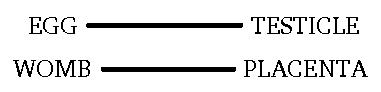
\includegraphics{../../pdf/intro21a.pdf}}

\item If the association crosses into another semantic field (e.g., if it is between a bodypart and a non-bodypart), the
non-bodypart point is labeled with small letters, e.g.:

\XeTeXpdffile "../../pdf/intro21b.pdf" 
% \resizebox{\columnwidth}{!}{
\includegraphics{../../pdf/intro21b.pdf}}

\item Antonymic associations (cases where the etymon has acquired opposite
meanings) are diagrammed by a curved \textit{yin-yang} type of line, e.g.:

\XeTeXpdffile "../../pdf/intro21c.pdf"
% \resizebox{\columnwidth}{!}{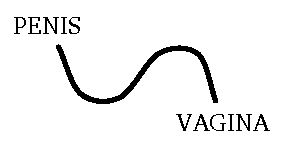
\includegraphics{../../pdf/intro21c.pdf}}

\item Compounds are diagrammed by a pitchfork-like symbol, with the two
constituents appearing at the points of the fork, and the overall meaning of the
compound indicated at the tip of the handle, e.g.:

\XeTeXpdffile "../../pdf/intro21d.pdf" 
% \resizebox{\columnwidth}{!}{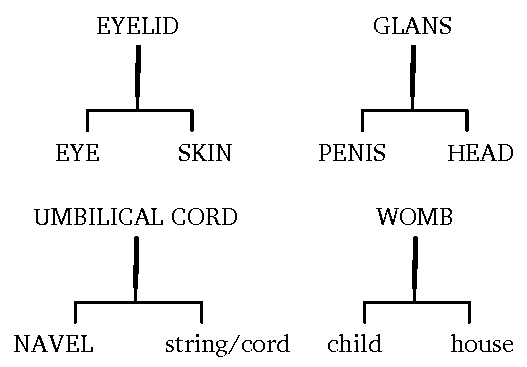
\includegraphics{../../pdf/intro21d.pdf}}

\end{enumerate}

The same convention with respect to capital vs.\ small letters applies to
compounds. In cases where several different combinations of morphemes are attested in compounds with the same meaning, graphic constraints sometimes require geometric reorientations of the pitchfork, e.g.

\XeTeXpdffile "../../pdf/intro21d2.pdf"
% \resizebox{\columnwidth}{!}{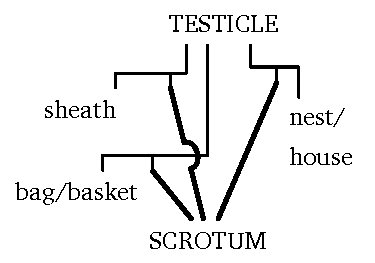
\includegraphics{../../pdf/intro21d2.pdf}}

The category of “reproductive bodyparts” is construed broadly to include
related verbs (e.g., KISS, SUCK, LOVE, SQUIRT). This volume also includes some
non-bodypart terms which frequently appear in compounds with etyma referring to
the reproductive system. See especially Ch.~IX, ‘Body fluids’.



More complex flowcharts have been constructed for the associations of SKIN, based on the analysis of XYZ etyma with that meaning. These are presented in Figs.~XYZ and PQR, in both “landscape” and “portrait” formats:\footnote{As a desideratum for the future, one might envision three-dimensional semantic diagrams like those used to model molecules in organic chemistry!}

[insert skin charts here]

In all language families, semantic associations/variation is much less structured than phonological variation. Sometimes the same unexpected semantic association is found in widely different language families, e.g.\ BRAIN and MARROW, exemplified both in IE and TB.\footnote{See JAM 1987 (VSTB), pp.~182–3, 203.} Other associations seem to be confined to a particular family, e.g.\ YEAST and SALT, so far discovered only in TB.\footnote{See 2003a (HPTB:34), and JAM 2003b. Yeast is traditionally used for brewing liquor rather than for baking bread in East and SE Asia. Both salt and yeast are efficacious substances that have dramatic effects on the taste of food or drink; their lack renders the food or drink insipid. Cf.\ Proto-Kuki-Naga \textbf{*m-tsyi} ‘salt’ and Jingpho \textbf{mətsi}, Lahu \textbf{dî} ‘yeast’ (Lahu voiced initials come from *prenasalized ones).}

The vagaries of semantic history occasionally result in strange allofamic bedfellows, e.g.\ Eng.\ \textbf{black} and \textbf{blank}, from the same PIE root \textbf{*bhel-} SHINE/FLASH/BURN/SHINING WHITE AND VARIOUS BRIGHT COLORS, or Eng.\ \textbf{science} and \textbf{shit} < \textbf{*skei-} CUT/SPLIT (AHD 58–9).

Given this unpredictability, how much semantic latitude is prudent in
our etymologies, and under what circumstances can semantic leaps be
plausibly justified? On the wild side we have megalo-comparative
fantasies with implausible semantic associations offered which are
totally unsupported by reasonable phonological correspondences or
areal semantic tendencies, as in Jan Braun’s Sumerian and
Tibeto-Burman (2001), in which he claims genetic connections between
pairs of words like the following:

\begin{tabular}{l l}
		\textit{Sumerian}		&		\textit{Written Tibetan}\\
		\textbf{gim} ‘axe’		&		\textbf{ḥgem-pa} ‘destroy’\\
		\textbf{alad} ‘protective demon’	&	\textbf{lad-mo} ‘imitation’\\
		\textbf{šinig} ‘tamarisk’	&		\textbf{snyigs-pa} ‘degenerated; grown worse’\\
		\textbf{peš} ‘three’	&		\textbf{gsum} ‘three’\\
\end{tabular}

Deciding how much semantic latitude to allow among putative cognates is
definitely an art rather than a science.\footnote{As in many other respects, Benedict was also a pioneer in the field of SE Asian areal semantics. Cf.\ his brilliant article “Semantic differentiation in Indo-Chinese” (1939).} Here as elsewhere a middle-of-the-road
approach is necessary, neither overly conservative nor too wildly speculative.

%Benedict 1939 was a pioneering article in the field of Southeast Asian areal semantics. At STEDT we have tried to make our semantic speculations as reasonable as possible. Each word in our lexical database is accompanied by a symbol which indicates the semantic field(s) to which it belongs. Within each point in semantic space, we attempt to trace the patterns of association for which there is evidence, by means of diagrams called ‘metastatic flowcharts’ in our jargon.3 FIGURES 7A and 7B are two attempts to indicate the attested semantic associations of SKIN in TB/ST.


\subsection{Regularity and variation}

Every spoken language is rife with variation on both the phonological and semantic planes, some of it rule-governed and some of it sporadic. Thus, despite the qualms of certain extreme neogrammarians, we must assume that this is true for proto-languages as well. It must be admitted that a lot of guesswork is involved in etymologizing
material from hundreds of languages and dialects at once, without having
established the “sound laws” in advance. The problems are especially acute when
comparing phonologically depleted languages with those having richer syllable
canons. When there is a partial phonological similarity between distinct etyma
with the same meaning (e.g.\ \textbf{*sem} and \textbf{*sak}  ‘mind / breath’;
\textbf{*muːr} and \textbf{*muk}
‘mouth’; \textbf{*s-maːy} and \textbf{*s-mel} ‘face’;
\textbf{*s-r(y)ik} and \textbf{*s(y)ar} ‘louse’), it is not
easy to decide by simple inspection to which etymon we should assign a
phonologically slight form in a daughter language (e.g.\ \textbf{sɒ} ‘mind’,
\textbf{mɔ̂} ‘mouth’,
\textbf{hmɛ} ‘face’).


There is a dialectical relationship between synchronic data and sound laws.
The “laws” are derived by inference from the data in the first place, but once
proto-forms are reconstructed, they can be used to guide us in our hunt for
cognates in languages not yet examined (even if they have undergone semantic
change). Almost every TB/ST etymology so far proposed presents problems and
complications—irregularities—in some language or other, which is par for
the course even in the much better known Indo-European family. Part of our task
is to indicate where the exceptions, problems, and irregularities lie, in the
hope that they can ultimately be explained.\footnote{The computer can be very
useful in deciding between alternative etymologies. Once “sound-laws” have been
formulated, computer checking can test whether a particular reconstruction
follows the laws, identifying inconsistencies in the reflexes of the same
proto-element in a given language. Such a methodology has been applied to the
Tamangic languages, using the “reconstruction engine” developed by J.B.\ Lowe at
STEDT in collaboration with Martine Mazaudon and Boyd Michailovsky during their
sojourns at Berkeley as visiting scholars (1987–89, 1990–91).} The concept of
“regularity” itself is by no means simple, nor does it mean the same thing to
different scholars.\footnote{See Matisoff 1992 (“Following the marrow”) and
1994a (“Regularity and variation”).}


Those who lack what I have called “Proto-Sprachgefühl”\footnote{See
Matisoff 1982.} can produce abstract, formulaic reconstructions bristling with
strange symbols but devoid of any phonetic or typological
plausibility.\footnote{Recent examples of this genre include Sedláček
1970; Weidert 1975, 1979, 1981, 1987; \citealt{PS-STL}; Sagart 2007.} 
Given sufficient semantic latitude and proto-forms that are complex enough, one
can formulate “sound laws” in such a way that they appear completely regular and
exceptionless. At an extreme level we find “megalocomparative” proposals of
genetic relationship that turn received notions upside down (e.g.\ Sino-Mayan,
Sino-Caucasian, Sino-Austronesian, Japanese-Dravidian), and which can lead the
unwary down fruitless paths, obscuring the differences among cognates,
borrowings, and chance resemblances.\footnote{See Matisoff 1990a (“On
megalocomparison”). Megalocomparison has the apparent advantage of
non-falsifiability, since, as Haudricourt has observed, one can never prove that
any two languages are not related. But non-falsifiable hypotheses are not
scientific. When presented with alternative non-falsifiable proposals it is
impossible to choose among them.} Various tricks of analysis that I have lumped
under the rubric of “proto-form stuffing” can help the Nostraticist or
Sino-Mayanist convince himself that his fantastical comparisons are “perfectly
regular”. Paradigmatically, one can multiply the number of proto-phonemes. If
you reconstruct 35 proto-vowels, any anomalous vowel correspondence can be
regarded as “regularly reflecting” a separate proto-vowel. Syntagmatically, if
you reconstruct etyma like \textbf{*mrgsla,} and the monstrous proto-cluster
\textbf{*mrgsl-}
occurs only in a single etymon, any set of reflexes in the daughter languages
can be said to be “regular”.\footnote{This is actually the proto-form offered
in Weidert 1981:25 for an etymon meaning ‘spirit, ghost, shadow’ (reconstructed
as \textbf{*m-hla} in \textit{STC} \#475). As I have observed (Matisoff 1982:22), “It is always
possible and sometimes necessary to invent an \textit{ad hoc} explanation for an
anomalous case. It is even true that some such \textit{ad hoc} ‘solutions’ are more
plausible than others. The only harm is in deluding oneself that an explanation
which covers only a single case establishes a ‘regularity’.”}


The time-depth of PST is perhaps 6000 years B.P., about at the limits of the
comparative method. We can hardly afford to insist on “perfect regularity” of
correspondence among our putative cognates. But instead of resorting to
“proto-form stuffing” to try to explain away problems, what is needed is an
explicit theory of variational phenomena. TB and ST etyma, like those of other
language families, are not independent isolated entities, but stand in complex
phonosemantic relationships with each other. It has been recognized for a long
time that words in Chinese and TB languages participate in morphophonemic groups
of partially resemblant forms that have been called “word families”.\footnote{See the pioneering study of Karlgren (1933), “Word families in Chinese”.}  In
Matisoff 1978 (\textit{VSTB}) I developed the notion of the \textit{allofam},
or individual member
of a word-family, and advocated the formulation of “allofamic reconstructions”
that accommodated all the well-attested variants deemed to descend from the same
proto-word-family. The symbol \STEDTU{⪤} was introduced to symbolize an allofamic
relationship between variant forms, i.e., “A \STEDTU{⪤} B” means that “A and B are
synchronic allofams of each other”, while “*A \STEDTU{⪤} *B” means that there is a
word-family relationship between A and B at the proto-level.\footnote{This
symbol \STEDTU{⪤}, a combination of  >  ‘goes to’ and < ‘comes from’, is meant to suggest
that neither variant is necessarily deemed to have temporal priority, but that
both must be set up to account for attested forms. Other related symbols are A~\STEDTU{↮}~B “A is not an allofam of B,” and A~\STEDTU{↭}~B “is A an allofam of B?”}


Needless to say, extreme care must be used in claiming that different forms
are variants of the same etymon. Allofamic theory must be applied in a
controlled and constrained way.\footnote{See the extended discussion in Ch.~XII
of \textit{HPTB} (pp.~491–534), “Allofamic variation in  rhymes”.} Not everything may be
said to vary with everything else! It is sometimes quite difficult to decide
whether partially resemblant forms represent separate etyma or whether they are
merely allofams of the same word-family. Not only must each proto-allofam fit
our canonic template (above section 4), but the type of variation posited must be
abundantly replicated in other examples. We do not attempt to
conceal such uncertainties, but frequently entertain the possibility that etyma
set up as independent might actually be co-allofams, or \textit{vice versa}.

\subsection{Notational conventions and pan-allofamic formulas}

The best attested patterns of variation in ST/TB are all exemplified in the
etymologies of this volume. They include the following:

\begin{enumerate}
\item %(a)
Voicing vs.\ voicelessness of the initial consonant:\footnote{Nothing is
more common in TB word families than variation of voicing in initial consonants,
largely due to the pervasive influence of prefixes on the manner of the initial.
 This is in sharp contrast to the situation in Indo-European or Austronesian, where such
variation in manner is quite rare, and is usually not tolerated in
reconstructions.}\nopagebreak[4]

\begin{tabular}{lll}
\textbf{*gop} \STEDTU{⪤} \textbf{*kop}	&(11a)	&HATCH/INCUBATE/COVER\\
\textbf{*prat} \STEDTU{⪤} \textbf{*brat}	&(75)	&BREAK/WEAN\\
\textbf{*tuŋ} \STEDTU{⪤} \textbf{*duŋ}	&(44a)	&NAVEL\\
\end{tabular}

\item %(b)
Variation between fricative and affricate:

\begin{tabular}{lll}
\textbf{*(t)sum}	&(45)		&NAVEL\\
\textbf{*(t)sip} \STEDTU{⪤} \textbf{*(t)sup} &(107)	&NEST/WOMB/SCROTUM\footnotemark\\
\end{tabular}
\footnotetext{This etymon also illustrates (f), below.}

\item %(c)
Presence vs.\ absence of medial \textbf{-y-}:

\begin{tabular}{lll}
\textbf{*b(y)at}	&(81)		&VAGINA\\
\textbf{*l(y)ap}	&(151)		&COPULATE\\
\end{tabular}

A special case of this pattern is the alternation between dental and palatal fricatives
and affricates:

\begin{tabular}{lll}
\textbf{*s(y)ok}	&(61)		&DRINK/SUCK/SMOKE\\
\textbf{*dz(y)əw}	&(56)		&BREAST/MILK\\
\textbf{*ts(y)uːŋ}	&(44b)		&NAVEL\\
\end{tabular}

\item %(d)
Variation between labial stop and labial semivowel:

\begin{tabular}{lll}
\textbf{*pu} \STEDTU{⪤} \textbf{*wu} 	&(1a, 1b)		&EGG\\
\textbf{*pam} \STEDTU{⪤} \textbf{*wam}	&(98a, 98b)	&WOMB/PLACENTA/NEST\\
\end{tabular}

\item %(e)
Variation between different prefixes:

\begin{tabular}{lll}
\textbf{*r-ga} \STEDTU{⪤} \textbf{*N-ga} \STEDTU{⪤} \textbf{*d-ga} \STEDTU{⪤} \textbf{*s-ga} &(141)	&COPULATE/LOVE/WANT\\
\textbf{*n-tow} \STEDTU{⪤} \textbf{*s-tow} &(3)		&EGG\\
\textbf{*m-ŋal} \STEDTU{⪤} \textbf{*l-ŋal} &(100)		&WOMB/PLACENTA\\
\end{tabular}

\item %(f)
Variation between \textbf{-u-} and \textbf{-i-} in closed syllables:

\begin{tabular}{lll}
\textbf{*dul} \STEDTU{⪤} \textbf{*dil} 		&(2b)	&EGG/TESTICLE\\
\textbf{*m-dzup} \STEDTU{⪤} \textbf{*m-dzip}	&(55)	&SUCK/SUCKLE/MILK/KISS\\
\textbf{*tsyur} \STEDTU{⪤} \textbf{*tsyir}	&(66)	&MILK/SQUEEZE/WRING\\
\end{tabular}

\item %(g)
Variation between medial \textbf{-ya-} and \textbf{-i-}:

\begin{tabular}{lll}
\textbf{*s-riŋ} \STEDTU{⪤} \textbf{*s-ryaŋ} &(39)	&LIVE/ALIVE/GREEN/RAW/GIVE BIRTH\\
\textbf{*s-nik} \STEDTU{⪤} \textbf{*s-nyak} &(124)	&PENIS/COPULATE\\
\textbf{*b-rim} \STEDTU{⪤} \textbf{*b-ryam} &(46)	&NAVEL/UMBILICAL CORD\\
\end{tabular}

\item %(h)
Alternation between medial \textbf{-wa-} and \textbf{-u-}:

\begin{tabular}{lll}
\textbf{*tsyul} \STEDTU{⪤} \textbf{*tsywal} &(105)	&WOMB/PLACENTA\\
\end{tabular}

\item \label{itm:hom-var} %(i)
Alternation between final homorganic stops and nasals:\nopagebreak[4]

\begin{tabular}{lll}
\textbf{*glim} \STEDTU{⪤} \textbf{*glip} 	&(15)	&BROOD/INCUBATE EGGS\\
\textbf{*s-nəwn} \STEDTU{⪤} \textbf{*s-nəwt} &(53c)	&BREAST/MILK/SUCK\\
\textbf{*tsiŋ} \STEDTU{⪤} \textbf{*tsik} &(78)	 	&VAGINA\\
\end{tabular}
\end{enumerate}


As some of the above examples illustrate, some roots show more than one type
of variation. When a posited allofamic reconstruction (e.g.\ \textbf{*sir} \STEDTU{⪤} \textbf{*sit} (6)
EGG) does not fall into a well-attested variational category, I comment on it. 
Handel makes similar remarks with respect to some of my TB comparisons with OC.


Occasionally, when the phonosemantic variation among the allofams is
considerable, and when each variant is amply attested, we split up the
presentation of the data into subroots that are designated by the same number
but with different lower case letters, e.g.: \textbf{*p-wu} (1) EGG is split into \textbf{*wu}
(1a) and \textbf{*pu} (1b);
\textbf{*m/s-la(ː)y} \STEDTU{⪤} \textbf{*s-tay} (40) NAVEL/CENTER/SELF is split into
\textbf{*m/s-la(ː)y} (40a) and \textbf{*s-tay} (40b);
\textbf{*m-ley} \STEDTU{⪤} \textbf{*m-li} \STEDTU{⪤} \textbf{*m-ney} (114) PENIS is
broken down into \textbf{*m-ley} \STEDTU{⪤} \textbf{*m-li} (114a)
and \textbf{*m-ney} (114b).


As I put it 42 years ago, “We must steer an Aristotelian middle path between
a dangerous speculativism and a stodgy insensitivity to the workings of
variational phenomena in language history.”\footnote{Matisoff 1972b (“Tangkhul
Naga and comparative TB”), p.~282.}

\subsection{Parallel but surprising examples}

Despite our concern with variational phenomena, we are always on the lookout for “sound laws” that can be established on the basis of parallel examples. A particularly striking sample is displayed in Figure \ref{ay}, which demonstrates that PTB *prefixed laterals before the rhyme \textbf{*-əy} developed into Lahu syllables with initial \textbf{h-} and the vowel \textbf{-ɔ}:

\begin{figure}
\caption{Lahu Reflexes of \textbf{-əy} after complex laterals}
\begin{tabular}{l l l l l l l}
 & Old Burmese & Lahu & Akha & Jingpho & WT & Proto-TB\\
‘wind’ & \textbf{le} & \textbf{mû-hɔ} & \textbf{} & \textbf{būŋ-lī} & \textbf{rdzi} & \textbf{g-ləy}\\
‘boat’ & \textbf{hle} & \textbf{hɔ-lɔ̀ʔ-qō} & \textbf{} & \textbf{lī} & \textbf{} & \textbf{m-ləy}\\
‘heavy’ & \textbf{lê} & \textbf{hɔ̂ ve} & \textbf{} & \textbf{lī} & \textbf{lći} & \textbf{s-ləy-t}\\
‘grandchild’ & \textbf{mliy > mrê} & \textbf{hɔ̄-ɛ̄} & \textbf{ø̀-pà} & \textbf{məlī} & \textbf{} & \textbf{b-ləy}\\
‘four’ & \textbf{lê} & \textbf{ɔ̂} & \textbf{ø̀} & \textbf{məlī} & \textbf{bźi} & \textbf{b-ləy}\\
‘bow/sling’ & \textbf{lê} & \textbf{hɔ̂-ma} & \textbf{ca-ø̀} & \textbf{ləlī} & \textbf{gźu} & \textbf{d/s-ləy}\\
\end{tabular}
\end{figure}

Yet even in this beautiful example there is an exceptional reflex in the Lahu word for ‘four’, which lacks initial \textbf{h-}. Surely this slight irregularity does not impugn the whole “sound law”, although it must be pointed out with hopes that it can ultimately be explained.\footnote{This exceptional Lahu reflex is reminiscent of Latin \textit{\=anser} ‘goose’ < PIE \textbf{*g\textsuperscript{h}ans-}, since the expected Latin reflex of \textbf{*gh-} is \textit{h-}. This irregular vowel-initial Latin form is usually described as a “cockneyism.”} Parallelism of variational patterns is very welcome, both within a language and across languages. See figure XYZ, which exemplifies the same pattern of variation between homorganic final stop and nasal (\#\ref{itm:hom-var} above) in Chinese and Lahu, two quite distantly related languages. After palatal initials, WT fairly regularly has \textit{-u} corresponding to front vowels in other languages. See HPTB: 192.


[[FILL IN VARIAtioN FOR SCATTER/POUR]]

\subsection{Notational conventions with respect to variation}

A few notational conventions with respect to my PTB reconstructions should
be mentioned:
\begin{itemize}
\item Variant reconstructed forms are indicated in several ways. They are usually
\mbox{written} with the ‘allofam symbol’ \STEDTU{⪤} between them, e.g.: \textbf{*glim} \STEDTU{⪤} \textbf{*glip}
BROOD~/ INCUBATE; \textbf{*s-riŋ} \STEDTU{⪤} \textbf{*s-r(y)aŋ} LIVE / ALIVE / GREEN / RAW / GIVE BIRTH.
Sometimes, however, I use an alternative notation with parentheses, e.g.: \textbf{*(t)si}
COPULATE/LOVE; this is equivalent to \textbf{*si} \STEDTU{⪤} \textbf{*tsi}.  Slashes may also be used,
e.g.\ \textbf{*p/buk} \STEDTU{⪤} \textbf{*p/bik} BORN/GIVE BIRTH; this is equivalent to
\textbf{*puk} \STEDTU{⪤} \textbf{*buk} \STEDTU{⪤} \textbf{*pik} \STEDTU{⪤} \textbf{*bik}.
Finally, still another way of indicating proto-variation is by means of a
‘vertical reconstruction’, e.g.:

\begin{quote}
*\textbf{\begin{tabular}[c]{c}t\\d\\\end{tabular}uŋ}  NAVEL.
This means the same as \textbf{*tuŋ} \STEDTU{⪤} \textbf{*duŋ}.
\end{quote}


\item Parentheses are especially appropriate for those frequent cases where there is
variation or indeterminacy between dental and palatal fricates; in fact that is
one of my principal motivations for writing the palatal series as sequences of
dental plus \textbf{-y-},
rather than writing them with \textit{ha\v{c}eks} or grave accents, e.g.:

\begin{quote}
\begin{tabular}{lll}
\textbf{*ts(y)uːŋ}	&NAVEL / CENTER		&(= \textbf{*tsuːŋ} \STEDTU{⪤} \textbf{*tšuːŋ)}\\
\textbf{*s(y)ok}	&DRINK / SUCK / SMOKE	&(= \textbf{*sok} \STEDTU{⪤} \textbf{*šok)}\\
\end{tabular}
\end{quote}

\item Etyma which show variation between initial \textbf{*p-} and \textbf{*w-} are reconstructed with
the morphophonemic symbol \textbf{*pʷ-,} which is roughly equivalent to treating the stop
element as a prefix (\textbf{*p-w-}).\footnote{For extended discussion of this issue,
see Matisoff 2000a.} Thus, a reconstruction like \textbf{*pʷu} EGG~/ BIRD~/ ROUND OBJECT
implies the existence of two sub-roots, \textbf{*pu} and \textbf{*wu,} whatever the ultimate
explanation for this variation might prove to be.

\item In the original version of Benedict 1972 (henceforth \textit{STC}, ca.~1943), Benedict reconstructed two PTB high
long vowels \textbf{*-iy} and \textbf{*-uw,} contrasting with the much less frequent short high
vowels \textbf{*-i} and \textbf{*-u.}  In the published version (1972) he modified the
reconstruction of these long vowels to \textbf{*-əy} and \textbf{*-əw,} a practice which I follow
myself. Occasionally, however, when the evidence does not permit us to decide
between a long and a short high proto-vowel, it is convenient to revert to the
earlier notation, with parentheses, e.g.\ \textbf{*b-ni(y)} ‘petticoat’ (\textit{STC} \#476);
\textbf{*sru(w)} ‘relative’ (\textit{STC} p.~108).
\end{itemize}

In cases where an etymon exhibits several different variational patterns, it is often advantageous to display these simultaneously in complex expressions that we call pan-allofamic formulas or “PAF’s” for short. A typical example is provided in Figure XYZ, presented in vertical format.

						
				Fig.~XYZ A typical PAF

A PAF is merely a convenient and concise way of representing several types of variation at once. In this cace they include (a) different prefixes attested with the root; (b) voicing alternation and lenition of the labial root-initial; (c) variation between the high vowels \textbf{-u-} and \textbf{-i-}; (d) evidence for long vowels in some reflexes; (e) presence or absence of a final velar stop. All of these variational patterns are directly instantiated in the various daughter languages. When necessary, such PAF’s are broken down into their individual allofams, with each supporting form assigned to a particular variant.

To avoid misunderstandings, several points must be made with respect to our PAF’s:

PAF’s are to be sharply distinguished from “pseudo-micritizing devices” for making \textit{ad hoc} comparisons look regular. Extreme examples of this approach are Benedict’s “split cognates” in Austro-Tai, where purported reflexes of the same etymon need have no proto-phoneme in common, e.g.\ 
\begin{quote}
DOG \hfill Proto-Austro-Tai \textbf{*[wa]k\d{l}əwm[a]} > Proto-Tai \textbf{*hma}, Proto-Hmong-Mien \textbf{*klu} (1975:272–3)
\end{quote}

\begin{itemize}
\item Not all mathematically possible variants provided for in a PAF are necessarily needed to cover all the reflexes that have been found. Thus, strictly speaking, Fig.~XYZ (BELLY/STOMACH) would permit 72 allofams: 3 prefixes (\textbf{*s-}, \textbf{*ʔ-}, or zero\footnote{The fact that many daughter languages show no trace of a prefix is indicated by the dashes in the PAF.}), $\times$ 3 root-initials $\times$ 2 vowels $\times$ 2 degrees of vowel length $\times$ 2 codas (zero or \textbf{*-k}). Certain mutual dependencies are not indicated in Fig.~XYZ, e.g.\ the fact that the alternation between \textbf{-u-} and \textbf{-i-} is only found in closed syllables, i.e.\ in syllables where there is evidence of final \textbf{-k}.

\item A PAF makes no claims about the relative antiquity of the various allofams that it represents. Such judgments may sometimes be inferred from the notes accompanying our etymologies, where the relative frequency and subgroup-distribution of the variants are usually detailed.

\item It may well turn out that certain variational patterns that have been observed reflect some deeper underlying regularity yet to be discovered. As discussed above, one way to attack an explanation based on variation is to propose a new proto-entity. Thus, e.g., we could reconstruct all etyma showing \textbf{-u-} \STEDTU{⪤} \textbf{-i-} variation with a special proto-vowel, say *barred eye. This “stuffing” of the proto-inventory buys us little, however, and I prefer simply to document the variational patterns which are well-documented, leaving them for future comparativists to evaluate.
\end{itemize}

\subsection{Similarities and differences between Tibeto-Burman and Indo-European patterns of variation}

Every spoken language is rife with variation on both the phonological and semantic planes, some of it rule-governed and some of it sporadic. Thus, despite the qualms of certain extreme neogrammarians, we must assume that this is true for proto-languages as well.

\subsubsection{Prefixal variation}

To have different prefixes attached to the same root is an extremely common phenomenon in TB, 
partly because prefixes may arise from the reduction of the first syllables of compounds (see ANT in Fig.~XYZ above), and also because certain TB languages seem to prefer a particular prefix to generalize throughout large parts of the lexicon.  Consonantal prefixes play a very minor role in IE etymologies. The only example I can think of is the s-mobile, a prefixal \textbf{*s-} that appears with a certain root in some languages but not in others with a certain root in some languages but not in others, e.g.\ PIE \textbf{*(s)teg-} ‘cover’ > Lat.\ \textit{tegō}, German \textit{decken}, OE {{\th}eccan}, but Greek \textit{stegō} and Russian \textit{stog}.\footnote{A good list of these roots is to be found in the index to the \textit{Lexikon der indogermanischen Verben} \citep{Rixetal2001}.}

\subsubsection{Manner of articulation of the root-initial}

As noted above, variation in the voicing of initial consonants is pervasive in TB, largely due to the influence of prefixes, which in many instances have disappeared, leaving only indirect traces. Thus the voiced series of obstruents in Lahu (/b d j g/) has been demonstrated to derived from Proto-Lolo-Burmese *prenasalized initials, which still survive as such in many Loloish languages like Luquan and Nasu (see JAM 1972 [TSR]).
In Indo-European, on the other hand, a discrepancy in voicing can sometimes be a fatal objection to a candidate for cognacy (see note XYZ, above).


%\subsubsection{Manners of initial consonants}
%In ST/TB variation in the manner of articulation (voiced or not, aspirated or not) of initial consonants is commonplace, largely due to the effect of prefixes. This is not so in Indo-European or Austronesian, where a voicing discrepancy can be a fatal objection to an etymology.

\subsubsection{Alternation between initial labial stop and w-}
In as many as 20 TB etymologies, some languages have a labial stop while others have \textbf{w-} (even though the “regular” correspondences are between  stops and stops and semivowels and semivowels); e.g.\ PIG WT \textbf{phag}/WB \textbf{wak}. This phenomenon, which I have called “extrusional”, occurs mostly before the vowel \textbf{-a-}.\footnote{See \citealt{JAM2000a}.}

\subsubsection{Vocalic alternations}
Conversely, vowel alternations (“ablaut” or “gradations”) are thoroughgoing and well-structured in IE, but quite sporadic in ST/TB, either confined to particular languages (e.g.\ Written Tibetan), or due merely to phonetic factors, without semantic content (e.g.\ alternation between medial \textbf{-i-} \STEDTU{⪤} \textbf{-u-}, especially in the environment of a labial $\textrm{C}_i$ and/or $\textrm{C}_f$. Even less phonetically motivated is the variation between \textbf{-i-} \STEDTU{⪤} \textbf{-ya-} found in several roots, notably EYE \textbf{*mik} \STEDTU{⪤}  \textbf{*myak}. Very occasionally a single etymon exhibits both types of alternation, e.g.\ BODY HAIR \textbf{*mul} \STEDTU{⪤} \textbf{*mil}  \STEDTU{⪤} \textbf{*myal}; FLY \textbf{*pur} \STEDTU{⪤} \textbf{*pir} \STEDTU{⪤} \textbf{*byar}.

\subsubsection{Variation between homorganic final stops and nasals}
This is common both in Chinese and TB, perhaps due to the influence of suffixes which have since disappeared; but this phenomenon is unknown in IE. See Fig.\ XYZ, above (SCATTER/POUR).

\subsubsection{Tonal variations}
Nothing is more common than for a ST/TB etymon to show tonal variation, either within a single language, or within a single subgroup, or across subgroups. These variations may be highly structured, even rule-governed (with clear conditioning), or they may be quite sporadic. Nevertheless tones usually do correspond very well within a subgroup, so that tonal anomalies must receive special attention. Tonally impoverished IE, on the other hand, must do without this sort of correspondence (except perhaps with respect to the pitch accents of Greek and Sanskrit, which sometimes do correspond regularly).

%Here is a PAF (in vertical format) which illustrates several of the types of variation just mentioned:
%BELLY/STOMACH
%			p
%		*s-		u
%			b		(?)	(k)
%		*?-		i
%			w
	
\subsubsection{Root extensions/augments in final position}
One variational feature shared by both TB and IE is the phenomenon of extra consonants tacked onto the end of a root, with no clear reason for it. First a couple of examples from TB:

		
TONGUE/LICK
\begin{tabular}{l l l l l l}
 & & & & & \textbf{(w)}\\
\textbf{*m-} & & & & & \\
 & & & & & \textbf{(y)}\\
 & \textbf{l} & \textbf{(y)} & \textbf{a} & \textbf{(?)} & \\	
\textbf{s-} & & & & \textbf{(m)}\\
 & & & & & \textbf{(k)}\\
\end{tabular}



FIRE/BURN/KINDLE/ROAST

\begin{tabular}{l l l l}
\textbf{*p} & & \textbf{r}\\
 & \textbf{w} & \textbf{l}\\
\textbf{b} & a & \\	
 & \textbf{y} & \textbf{m, n, ŋ}\\	
h & & t\\
\end{tabular}

A very similar example from Indo-European involves the morpheme \textbf{*wer-} TURN/BEND, called “the conventional basis of various Indo-European roots” (AHD: 76–77). See Figure XYZ.

FIGURE: \textbf{*wer-} TURN/BEND  “conventional basis of various Indo-European roots”  AHD 76–77:

\begin{enumerate}
\item \textbf{*wert-}	>	-WARD	(forward, toward, etc.) / Lat.\ \textit{vert-} (convert, revert, divert, etc.)

\item \textbf{*wreit-}	>	WREATH / WRITHE / WRATH

\item \textbf{*wergh-}	>	WORRY / WRING

\item \textbf{*werg-}	>	WRENCH / WRINKLE

\item \textbf{*wreik-}	>	WRY / WRIGGLE / WRIST / WRESTLE

\item \textbf{*wrib-}	>	RIBALD

\item \textbf{*werb-}	>	WARP

\item \textbf{*werp-}	>	WRAP / RHAPSODY

\item \textbf{*w\textsubring{r}mi-}	>	WORM
\end{enumerate}


V. More on the concept of word family: blood relatives vs.\ adoptive ones

According to the broad definition of “word family” adopted at STEDT, a family may include “blood relatives” (i.e.\ native words directly descended from an earlier stage of a given language), as well as words borrowed from a related language (“adoptive relatives”). It is the task of the analyst to distinguish these two types of family members. In TB, this problem is often acute, e.g.\ with respect to the Baic languages of Yunnan, which have been overwhelmed with different strata of loanwords from Chinese over the millennia. Indo-European also has countless examples of this mixed type of word family, as in Figure XYZ.

\begin{figure}
\caption{English reflexes of the PIE etymon \textbf{*wed-} \STEDTU{⪤} \textbf{*wod-} \STEDTU{⪤} \textbf{*ud-} WATER (adapted from AHD 73)}
\begin{enumerate}
\item Inherited Germanic material
\begin{enumerate}
\item  \textbf{*wod-\=or-}	[suffixed o-grade]
	> PGmc \textbf{*watar} > OE {\it w{\ae}tar} > WATER
\item \textbf{*w\={e}d-o-}	[suffixed lengthened grade]
  > PGmc \textbf{*w\=ed-} > OE {\it w{\ae}t}, {\it w\=et} > WET
\item \textbf{*wod-}	[o-grade]
	> PGmc \textbf{*wat-skan} > OE {\it w{\ae}scan}, {\it wacsan} > WASH
\item \textbf{*we-n-d-}	[nasalized form]
	> PGmc \textbf{*wintruz} ‘wet season’ > OE {\it winter} > WINTER
\item \textbf{*ud-ro}, \textbf{*ud-\textsubring{r}-}  [suffixed zero-grade]
	> PGmc \textbf{*otraz} > OE otor > OTTER
\end{enumerate}

\item Borrowings from other Indo-European languages
\begin{enumerate}
\item \textbf{*ud-\=or-}	[suffixed zero-grade]
	> Greek {\it hud\=or} ‘water’ > HYDRO- (including CLEPSYDRA, DROPSY)
\item \textbf{*u-n-d-\={a}-}	[suffixed nasalized zero-grade]
	> Latin {\it unda} ‘wave’ > UNDULATE, INUNDATE, ABOUND, REDUNDANT, SURROUND
\item \textbf{*ud-skio-}	[suffixed zero-grade]
	> Scot.\ and Ir.\ Gaelic {\it uisge} ‘water’ > {\it uisquebaugh} ‘eau de vie’ > WHISKEY
\item \textbf{*wod-\={a}-}	[suffixed o-grade]
	> Russ.\ {\it voda} ‘water’, with {\it -ka} ‘diminutive’ > VODKA
\end{enumerate}
\end{enumerate}
\end{figure}



%\subsection{Regularity and exceptions}

%Exceptionlessness vs.\ parallel examples.1  How many parallel examples do we need to establish “regularity”?  Are exceptions more to be tolerated in “core” than in “peripheral” vocabulary? In very favorable circumstances we might find several parallel examples that prove the validity of a correspondence that at first glance seemed most unlikely. See Figure XYZ.

%	FIGURE:  Lahu Reflexes of \textbf{*-əy} after complex laterals

%\begin{tabular}{l l l l l l l}

% &		Old Burmese &	Lahu &		Akha &	Jingpho & WT & Proto-TB\\
% ‘wind’	&	le	&	mx85-h?	& &  bx21-l?	&	rdzi &
% *g-l{\textschwa}y\\
%‘boat’	&	hle	&	h?-lx85?-q?	& &	l?	&	&	*m-l?y\\
%‘heavy’	&	lx85	&	h? ve	& &		l?	& l?i &	*s-l?y-t\\
%‘grandchild’ &	mliy > mr\=e &	h?-?		 & & ?-px85	m?l?
%“young man” & &	*b-l?y\\
%%‘four’	&	lx85	&	?	&	? &	m?l?	& b?i &	*b-l?y\\
%‘bow/sling’ &	lx85	&	h?-ma	& & ca-?	l?l?	& g?u\\
%2 &	*d/s-l?y\\
%\end{tabular}

%Problem: How to deal with Lahu ?, which lacks initial h-?
%Parallelism of variational patterns is a big plus, both within a
%language and across languages.  See FIGURE XYZ:
%

%	FIGURE:  Parallel patterns of variation in Lolo-Burmese and Chinese: SCATTER/POUR

%			PST/PTB *sywar > OC *sx85n  ?  *sx85t  and PLB *swan  ? *swat
%(1) PTB *sywar ‘flow/pour/scatter’
%	WT h?tshor-ba ‘escape; flow out, run over’; Lepcha t?hor ‘the pouring of water; Garo sol-a?
%	‘flow’; Dimasa di-sor ‘id.’; Jingpho x21n ‘flow (as tears, sweat, water poured on ground)’
%(2) PLB *swan  ? *swat
%	*swan?/?  > WB swan ‘pour out, spill, shed’, swx85n ‘pour upon, cast by pouring liquid into a
%	mold’; Lahu x21 ‘pour; sow broadcast; Akha s? ‘sow seeds, sj? ‘pour’; Mpi se? ‘sow broadcast’
%	*swat	>    Lahu ?x85? ‘pour, spill’; Akha sj?q; Sani sx23; Bisu x21t
%(3) OC  *sx85n  ?  *sx85t
%	*sx85n  >  ?  [GSR 156a-b] (Mand.\ sx85n) ‘disperse’
%	*sx85t   >  ?   [AD 767]  (Mand.\ s?, s?)  ‘scatter; let loose’

%For the ST/TB variational pattern of homorganic final stops and nasals, see below XYZ.


%\section{Variational phenomena}
%Allofam theory: since VSTB
%	The three symbols: 	A is an allofam of B
%				A is not an allofam of B
%				is A and allofam of B?

%* Isotopes are allofams of elements.


%. Patterns of phonosemantic variation in Tibeto-Burman vs.\ Indo-European3

	
	
%\subsection{Rectification/revision of reconstructions}
%
%As of January 2014, about XYZ\% of our etymologies have gone through the rectification process. We shall complete this task during the year-long no-cost extension of the current STEDT grants.

%We have nothing to apologize for in changing our reconstructions (look at all the revisions of Baxter/Sagart!). In our case, we’re not just rechewing the same old data in ever more implausible ways, but rather trying to accommodate all the new data that keep pouring in. 
%In cases where the reconstructions in this Final Product differ from those in HPTB or other previous publications, the FP wins (providing the etymon has been properly rectified).

%Etymological accuracy and rectification of possible errors
%	TBRS, Section 3.2, pp.~xxxviii-xl
%	HPTB, pp.~538–40

	
\subsection[Etymological accuracy and rectification of possible errors]{Etymological accuracy and rectification of possible errors}

Our STEDT etymologies have been undergoing a constant process of “rectification”, and may be roughly divided into three types: (a) those to be accepted as is; (b) those to be accepted with modifications; and (c) those to be rejected. 
As with all scientific hypotheses, our reconstructions are falsifiable in the light of new data or better analyses. 
There are all too many ways in which one can make etymological mistakes, and
I have been guilty of all of them at one time or another.\footnote{The discussion in this section is adapted from \textit{HPTB}, pp.~538–40.} 
A rough taxonomy of
errors would have to include the following:


\paragraph{Treating a loanword as native}

I was at first delighted when I ran across the Jingpho form \textbf{wéʔ-wū} ‘screw’,
since its first syllable looked like an excellent match with Lahu \textbf{ɔ̀-vɛ̀ʔ} ‘id.’,
for which I then had no etymology. Could this be a precious example of the rare
PTB rhyme \textbf{*-ek}? But the screw is hardly an artifact of any great antiquity, and
it would be \textit{prima facie} implausible that a root with such a meaning would have
existed in PTB. The truth quickly became apparent. The modern Burmese form for
‘screw’, \textbf{wɛ́ʔ-ʔu} (WB \textbf{wak-ʔu}), the obvious source from which both Jingpho and
Lahu borrowed these words, means literally “pig-intestine”.  The semantic
association is the corkscrew-like appearance of a pig’s small intestine. This
etymology is also interesting from the viewpoint of distinguishing native vs.\
borrowed co-allofams. The usual, native words for ‘pig’ in Jingpho and Lahu are
\textbf{wàʔ} and \textbf{vàʔ}, respectively; but the doublets borrowed from Burmese have front
vowels, as in spoken Burmese. Unless a native speaker of Jingpho knows Burmese,
s/he is unlikely to realize that the first syllable of \textbf{wéʔ-wū} means ‘pig’,
especially since this syllable is in the high-stopped tone, while ‘pig’ is
low-stopped. The native Lahu speaker is even less likely to recognize the source
of \textbf{ɔ̀-vɛ̀ʔ}, since the morpheme for ‘intestine’ has been completely dropped from
the original Burmese compound, rather like the way our word \textit{camera} (< Lat.\
‘room; chamber; vaulted enclosure’) is a shortening of the old compound \textit{camera
obscura} (“dark chamber”).\footnote{There is a difference in detail between the
two cases, however: the deleted ‘intestine’ is the head of the compound
“pig-intestine”, but the deleted \textit{obscura} is the modifier in the collocation
“dark-chamber”.}

\paragraph{Combining reflexes of unrelated roots}

When two forms bearing a semantic resemblance in a phonologically depleted
language differ only in tone, it is tempting to try to relate them. I once
entertained the possibility that such pairs of Lahu forms as \textbf{phu} ‘silver, money’
/ \textbf{phû} ‘price, cost’ and \textbf{mu} ‘high, tall’ / \textbf{mû} ‘sky’ were co-allofams, though they
can easily be shown to descend from quite separate etyma: \textbf{phu} < PTB \textbf{*plu} (\textit{STC} p.
89) / \textbf{phû} < PTB \textbf{*pəw} (\textit{STC} \#41);
\textbf{mu} < PTB \textbf{*mraŋ} (\textit{STC} p.~43) / \textbf{mû} < PTB \textbf{*r-məw}
(\textit{STC} \#488).\footnote{See Matisoff 1973b (\textit{GL}:29); such speculations were debunked in
the 2nd Printing (1982) of \textit{GL}, p.~675.}

\paragraph{Failure to recognize that separately reconstructed etyma are really co-allofams}

An opposite type of error is to overlook the etymological identity between sets
of forms, assigning them to separate etyma when they are really co-allofams.
Thus \textit{STC} sets up two independent PTB roots, both with the shape \textbf{*dyam}, one
meaning ‘full; fill’ (\textit{STC} \#226) and the other glossed as ‘straight’ (\textit{STC} \#227).
Yet it can be shown that the latter root also means ‘flat’, and that all
reflexes of \#226 and \#227 may be subsumed under a single etymon, with the
underlying idea being “perfection in a certain dimension”.\footnote{See Matisoff
1988b:4–9.}


Similarly, I was slow to recognize that two roots I had set up separately,
PLB \textbf{*dzay²} ‘cattle; domestic animal’ (Matisoff 1985a \#129)
and NE Indian \textbf{*tsaːy} ‘elephant;
cattle’ (\#143) are really one and the same.\footnote{I have argued that a
third root set up in Matisoff 1985a (\textit{GSTC} \#106), \textbf{*(t)saːy} \STEDTU{⪤} \textbf{*(d)zaːy} ‘temperament / aptitude / talent’, is also related, the common notion being ‘property (either material or
intellectual)’. See Matisoff 1985a:44–45; 1988b:10–13.}

\paragraph{Double-dipping}
This embarrassing situation occurs when an author inadvertently assigns the same
form in a daughter language to two different etyma, perhaps within the pages of
the same book, but more likely in separate articles. At different times I have
compared Chinese \textbf{chún} \TC{唇} ‘lip’ (OC \textbf{d̑i̯wən}) to both PTB \textbf{*dyal}
and \textbf{*m-ts(y)ul}, finally deciding in favor of the latter.\footnote{See \textit{HPTB}
9.2.1, 9.22(4), 9.2.4.}  It
is of course perfectly legitimate to change one’s mind, as long as one explains
why. The best course is to present the alternative etymologies together,
inviting the reader to choose between them.

\paragraph{Misanalyses of compounds}
A vast number of words in TB languages are di- or tri-syllabic compounds, a fact
which greatly complicates the task of etymologization. Many traps lie in wait
for the analyst, leading to potential errors of several kinds.

\subparagraph{Wrong segmentation}
This can happen when a form in an inadequately transcribed source is not
syllabified. The Pochury and Sangtam forms for ‘star’, transcribed as \textbf{awutsi}
and \textbf{chinghi}, respectively, in the little glossaries compiled by the
\textit{Nagaland
Bhasha Parishad},\footnote{Kumar et al., \textit{Hindi Pochury English Dictionary} (1972);
\textit{Hindi
Sangtam English Dictionary} (1973). Kohima: Linguistic Circle of Nagaland.}
 should
be segmented as \textbf{a-wu-tsi} and \textbf{ching-hi},
and not as \textbf{a-wut-si} and \textbf{chi-nghi}, as I
imprudently did in Matisoff 1980:21.


\subparagraph{Misunderstanding the meaning of a constituent}
A special case of this problem is mistaking an affix for a root, especially
likely to occur when no grammatical description exists for a language. Several
Naga languages have dissyllabic forms for ‘moon’ with similar final syllables,
e.g.\ Chang \textbf{litnyu}, Konyak \textbf{linnyu},
Phom \textbf{linnyü}, Sangtam \textbf{chonu}, Liangmai \textbf{chahiu}.
Yet these final elements do not constitute a new root meaning ‘moon’, as I had
originally guessed; rather they represent an abstract formative, ultimately
grammaticalized from a root \textbf{*n(y)u} ‘mother’, that occurs in nouns from all sorts
of semantic fields (e.g.\ Chang \textbf{chinyu} ‘center’,
\textbf{henyu} ‘ladder’, \textbf{lamnyu} ‘road’,
\textbf{pinyu} ‘snake’).\footnote{See Matisoff 1980 (“Stars, moon, spirits”), p.\ 35;
for the
suffixal use of morphemes meaning ‘mother’, see Matisoff 1991b (“The mother of all
morphemes”).}


\subparagraph{Choosing the wrong syllable of a compound for an etymology}
This can happen when two different syllables of a compound are phonologically
similar, especially if one is dealing with a poorly known language with depleted
final consonants, e.g.\ forms like Guiqiong Ganzi \textbf{tʃhə⁵⁵sɑ̃⁵⁵}
and Ersu \textbf{ʂɿ⁵⁵ji⁵⁵} ‘otter’.
Which syllables are to be ascribed to PTB \textbf{*sram}? 

%\paragraph{Semantic leaps}
%Deciding how much semantic latitude to allow among putative cognates is definitely an art rather than a science. Here as elsewhere a middle-of-the-road approach is necessary, neither overly conservative nor too wildly speculative. As a positive example of a promising new etymology involving a semantic leap, we may offer *m-t(s)i ‘salt / yeast’.\footnote{Above 3.3.1.} Phonologically the reflexes correspond perfectly well. On the other hand, the semantic association between ‘salt’ and ‘yeast’ has yet to be attested elsewhere, even though it has great initial plausibility. Both are efficacious substances that have dramatic effects on the taste of food or drink; their lack renders the food or drink insipid.\footnote{Yeast is used for brewing liquor rather than for baking bread in East and SE Asia.}

By its very nature, comparative/historical investigation of such a complex language family as TB/ST is an open-ended enterprise. As described above (FILL IN), changes continue to be made in the details of the STEDT reconstructive system,\footnote{Cf.\ the recent reinterpretation of the PTB mid-vowels \textbf{*-e(-)} and \textbf{*-o(-)} as rising and falling diphthongs (above FILL IN).} as well as in our conception of the subgrouping of the family.\footnote{Cf.\ the recent reevaluation of the genetic position of Jingpho, Luish and Nungish (above FILL IN).}

\subsection{Desiderata for the future}

I am acutely aware of the incompleteness of this Dictionary-Thesaurus. As noted in the Preface, we still have a long way to go before comparative/historical TB/ST studies are as advanced as they deserve to be. Despite the quickening pace of research, our knowledge of the various branches of this multifarious family remains highly uneven. With a few important exceptions,\footnote{These bright spots include Proto-Karen (Haudricourt, Jones, Solnit), PNN (French), Proto-Tani (J.\ Sun), Proto-Tamangic (Mazaudon), Proto-Kiranti (Michailovsky), Proto-Central Chin (VanBik), Proto-Lolo-Burmese (Burling, Matisoff, Bradley). See the References.} reliable reconstructions at the subgroup level are not yet available, so that “teleo-reconstruction” has to be resorted to.\footnote{See \citealt{PKB-TBT}.} Many more roots remain to be reconstructed at all taxonomic levels of the family.

Much remains to be done on the Chinese side as well, and we seem destined for a period of flux until the dust settles and competing reconstructions have sorted themselves out.

A large lacuna in this work is the lack of a systematic treatment of tone. This is not because the topic does not interest me, but rather because it merits a book-length treatment by itself. We are only just coming to appreciate the richness and variety of TB tone systems as more and more data become available.\footnote{For a rough typology of TB tone systems, see JAM 1999a. Weidert (1987) is an attempt to reduce all TB tone systems to a single proto-phonational contrast among clear, breathy, and creaky voice qualities, but is marred by an over-formalistic and disorganized presentation which renders it virtually incomprehensible. See the review by JAM (1994c).} The big questions are still open, especially the key issue of monogenesis vs.\ polygenesis: Can we reconstruct a single tonal system at the PTB level? At the PST level? If so, was this original system primarily phonational or melodic? Or are tonogenesis and tonoexodus cyclical processes, with tones having arisen repeatedly and independently in the various branches of TB, so that even if there was an “original” system, it can no longer be recovered?

Despite the fact that changes continue to be made in our reconstructions (see FILL IN above), STEDT continues to build upon previous research rather than repudiating it. 
Perpetual revolution gets to be fatiguing after a while.\footnote{As Leon Trotsky found to his cost in 1940.} Historical linguistics is a cumulative enterprise. Thanks to the foundation laid by pioneering scholars, especially Paul K.\ Benedict, a solid body of TB/ST etymological knowledge has been accumulated, in terms of which new etymologies must be evaluated. No longer can one get away with reconstructing whatever one pleases, no matter how typologically bizarre or adhoc or mechanistic the reconstruction might be.\footnote{Those who lack what I have called “Proto-Sprachgef\"uhl” (JAM 1982a) can produce reconstructions bristling with strange symbols but devoid of any phonetic or typological plausibility; see e.g.\ Sedl\'a\v{c}ek 1970; Weidert 1975, 1979, 1981, 1987; \citealt{PS-STL}.}

All in all, it is hard not to be optimistic about the future of TB/ST linguistics, as fieldwork opportunities increase and new generations of talented researchers enter the discipline. Eventually it seems inevitable that scholars throughout the world will share their information more and more, granting mutual access to their databases for the common good. On the other hand, too many TB languages are endangered, and may well disappear before they have been adequately recorded.

In any case, “the reconstruction of PTB is a noble enterprise, where a spirit of competitive territoriality is out of place. We should pool our knowledge and encourage each other to venture outside of our specialized niches, so that we begin to appreciate the full range of TB languages...”\footnote{JAM 1982a:41.}


%\subsection{Philosophical ruminations}

%Both phonological and semantic reconstructions are arts as well as sciences, arts which require a feel for proto-languages (what I have called Proto-Sprachgef\"uhl), as well as a commitment to “steer an Aristotelian middle path betwen a dangerous speculativism and a stodgy insensitivity to the workings of variational phenomena in language history.”1 

%We Tibeto-Burmanists need not apologize to Indo-Europeanists, or be envious of them. Even relative neophytes can make important discoveries in our field, which is a maximal contrast with the cutthroat world of Indo-European, where you can spend your whole life defending a single “new” etymology.

%I much prefer the maxim Errare humanum est to the dreadful judgment Falsum in uno, falsum in omnibus.

%It is admirable to correct one’s own mistakes, both typographical and analytical. We should indeed suffer from our errors, but also correct them at every opportunity. As STEDT goes off into the twilight, we are doing all we can to “rectify” our etymologies, accepting most of them without modification, but also revising many others, and throwing out a relatively small number of them altogether.

%Although it is admirable to change one’s mind for good reason, it is frivolous to change one’s reconstructions just for the sake of being different.

%It is admirable to evaluate the reconstructions of others critically, and to offer better alternatives if possible. But it is frivolous to make trivial changes in previously established reconstructions simply in order to call them one’s own.

%Cumulativity vs. perpetual revolution. Don’t throw out the baby with the bath-water. It is better to build on previous etymological work, rather than attempting to tear it all down and start over. Avoid Freudian patricidalism.

%Do not be discouraged as you stumble along from one half-truth to another in this marvelous enterprise we call etymologization.

%Etymology is an art as much as a science. But just as in any art, there are better and worse practitioners. We owe it to the field to be responsible and to hold ourselves to the highest standards of intellectual 
%honesty and collegiality.

%As STEDT goes off into the twilight, there are hopes that it will continue in a more 21st century way.  Creation of an international consortium: the interactive “Root Canal”.

%\section{Conclusion}
%One cannot very well end a book with the word “horse-leech”, and so a few concluding philosophical remarks seem appropriate. Perhaps the best way to organize this discussion is in terms of a set of adjectives with the -ive suffix.

%\subsection{Cumulative}

%In linguistics as in other disciplines, it is a constant temptation to try to overthrow the work of one’s predecessors, so that one’s own research will appear to be the {\it fons et origo} of the truth.\footnote{I have referred to this phenomenon in Freudian terms as “patricidal” (keynote address at the Summer Institute of the Linguistic Society of America, Ann Arbor 1973).}
%This tendency has been especially characteristic of generative grammar, where “theories of language” have a built-in planned obsolescence, with each new theory claiming to invalidate all previous ones.

%Historical linguists are hardly exempt from this primal urge for revolutionary novelty  the desire to be different just for the sake of being different. This can take many forms, some of them trivial and innocuous, like replacing a phonetic symbol in a previous reconstruction by a new but equivalent one; or changing the name of a subgroup of a language family.\footnote{Hence the proliferation of alternate names even for well-established subgroups like Lolo-Burmese (Burmese-Lolo, Yi-Burmese, Burmese-Yi, Burmese-Yipho, Yi-Myanmar, Myanmar-Yipho, etc.). T. Shintani has recently (2002) proposed the euphonious neologism “Brakaloungic” for Karenic.}
%More serious is the itch to carve out totally novel subgroupings,\footnote{I have called this “neosubgroupitis” (JAM 2000b “On Sino-Bodic”). Trying to establish higher-order combinations of TB subgroups is premature at best. Even Indo-Europeanists are still unable to do so unequivocally for their much better documented family. See the discussion in JAM 1978a (VSTB):1–12.} a process rather similar to the decennial gerrymandering of congressional districts in the House of Representatives. At an extreme level we find “megalocomparative” proposals of genetic relationship that turn received notions upside down (e.g.\ Sino-Mayan, Sino-Caucasian, Sino-Austronesian, Japanese-Dravidian), and which can lead the unwary down fruitless paths, obscuring the differences among cognates, borrowings, and chance resemblances.\footnote{See JAM 1990a (“On megalocomparison”). Megalocomparison has the apparent advantage of non-falsifiability, since, as Haudricourt has observed, one can never prove that any two languages are not related. But non-falsifiable hypotheses are not scientific. When presented with alternative non-falsifiable proposals it is impossible to choose among them.}

%Perpetual revolution gets to be fatiguing after a while.\footnote{As Leon Trotsky found to his cost in 1940.} Surely it is preferable to build on the past rather than to repudiate it. Historical linguistics is a cumulative enterprise. Thanks to the foundation laid by pioneering scholars, especially Paul K.\ Benedict, a solid body of TB/ST etymological knowledge has been accumulated, in terms of which new etymologies must be evaluated. No longer can one get away with reconstructing whatever one pleases, no matter how typologically bizarre or adhoc or mechanistic the reconstruction might be.\footnote{Those who lack what I have called “Proto-Sprachgef\"uhl” (JAM 1982a) can produce reconstructions bristling with strange symbols but devoid of any phonetic or typological plausibility; see e.g.\ Sedl\'a\v{c}ek 1970; Weidert 1975, 1979, 1981, 1987; Peiros \& Starostin 1996.}

%There is a dialectical relationship between synchronic data and sound laws. The “laws” are derived by inference from the data in the first place, but once proto-forms are reconstructed, they can be used to guide us in our hunt for cognates in languages not yet examined (even if they have undergone semantic change). Almost every TB/ST etymology so far proposed presents problems and complications  irregularities  in some language or other, which is par for the course even in the much better known Indo-European family. Part of our task is to indicate where the exceptions, problems, and irregularities lie, in the hope that they can ultimately be explained.

%The concept of “regularity” itself is by no means simple, nor does it mean the same thing to different scholars.\footnote{See JAM 1992 (“Following the marrow”) and 1994a (“Regularity and variation”).} The Nostraticist or Sino-Mayanist can convince himself that his fantastical comparisons are “perfectly regular”. Given sufficient semantic latitude and proto-forms that are complex enough, one can formulate “sound laws” in such a way that they appear exceptionless. Paradigmatically one can multiply the number of proto-phonemes. If you reconstruct 35 proto-vowels, any anomalous vowel correspondence can be regarded as “regularly reflecting” a separate proto-vowel. Syntagmatically, if you reconstruct etyma like *mrgsla, and the monstrous proto-cluster *mrgsl- occurs only in a single etymon, any set of reflexes in the daughter languages can be said to be “regular”.\footnote{This is actually the proto-form offered in Weidert 1981:25 for an etymon meaning ‘spirit, ghost, shadow’ (reconstructed as *m-hla in STC \#475). As I have observed, “It is always possible and sometimes necessary to invent an ad hoc explanation for an anomalous case. It is even true that some such ad hoc ‘solutions’ are more plausible than others. The only harm is in deluding oneself that an explanation which covers only a single case establishes a ‘regularity’.” (JAM 1982a:22).}

%As the alternative to such “proto-form stuffing”, one must have recourse to proto-variation, though in a controlled and constrained way. Not everything may be said to vary with everything else.\footnote{This issue is the major theme of JAM 1978a (VSTB).} This Handbook places special emphasis on variational patterns in TB/ST, and attempts to classify them according to how well attested they are.\footnote{Note the large percentage of PTB roots for which proto-variation is posited in the Index of Proto-Forms, below.} As I put it 30 years ago, “We must steer an Aristotelian middle path between a dangerous speculativism and a stodgy insensitivity to the workings of variational phenomena in language history.”\footnote{JAM 1972b (“Tangkhul Naga and comparative TB”):282.}

%The time-depth of PST is perhaps 6000 years B.P., about at the limits of the comparative method. We can hardly afford to insist on “perfect regularity”, though we must never settle for a roseate Greenbergian haze.\footnote{See Greenberg 1987, and my review of it (JAM 1990a).}


%\section*{A New Era}
%Although I feel that we are entering a new era of etymological
%responsibility in TB/ST studies  the bar has been raised, as it were
%I am not suggesting that we turn our field into a “tough neighborhood”
%like that of the Indo-Europeanists. In particular I hope we can avoid
%the “Gotcha!” attitude,\footnote{Non-American readers might need a
%  word of explanation here: “Gotcha” is an attempt to render the
%  colloquial pronunciation of “(I’ve) got you (now)!”, a triumphant
%  phrase used by someone who feels he has won an argument.} whereby if
%a single error, real or fancied, is found in an article or book, the
%whole work is impugned. This attitude is encapsulated in the dreadful
%maxim {\it Falsum in uno, falsum in omnibus}.\footnote{ “If one thing
% is wrong, it’s all wrong.” This was the approach of Miller’s
% (1974) bitter review of STC, in which he tried to kill the Conspectus just as it was born. In my “rejection” of his “Conspectus inspection” I characterized his strategy as follows: (a) make some criticism of a particular point, no matter how trivial, irrelevant or obfuscatory; (b) claim that tout se tient, and that the entire work stands or falls on the point in question; (c) beat the point elaborately to death; (d) avoid any substantive comments by pleading lack of space (JAM 1975a:157).}

%Historical linguists cannot afford to be too thin-skinned, as long as criticism is fair, constructive, and proportionate. As I have said in print, “I ask nothing better than to be corrected.”\footnote{JAM 1985b (“Out on a limb”):422.} Or again, “We can take comfort from our mistakes. Reconstruction of a proto-lexicon is a piecemeal process. It is hardly surprising that we stumble along from one half-truth to another, as we try to trace the [phonological and] semantic interconnections among our reconstructed etyma. We should not be discouraged if we barge off down blind alleys occasionally, or if the solution to one problem raises as many questions as it answers.”\footnote{JAM 1988a:13.}

%After all, a computerized etymological enterprise by its very nature is eminently revisable.

%\subsection{Desiderative}
%I am acutely aware of the incompleteness of this Dictionary-Thesaurus. As noted in the Preface, we still have a long way to go before comparative/historical TB/ST studies are as advanced as they deserve to be. Despite the quickening pace of research, our knowledge of the various branches of this multifarious family remains highly uneven. With a few important exceptions,\footnote{These bright spots include Proto-Karen (Haudricourt, Jones, Solnit), PNN (French), Proto-Tani (J.\ Sun), Proto-Tamangic (Mazaudon), Proto-Kiranti (Michailovsky), Proto-Central Chin (VanBik), Proto-Lolo-Burmese (Burling, Matisoff, Bradley). See the References.} reliable reconstructions at the subgroup level are not yet available, so that “teleo-reconstruction” has to be resorted to.\footnote{See Benedict 1973.} Many more roots remain to be reconstructed at all taxonomic levels of the family.

%Much remains to be done on the Chinese side as well, and we seem destined for a period of flux until the dust settles and competing reconstructions have sorted themselves out.

%A large lacuna in this work is the lack of a systematic treatment of tone. This is not because the topic does not interest me, but rather because it merits a book-length treatment by itself. We are only just coming to appreciate the richness and variety of TB tone systems as more and more data become available.\footnote{For a rough typology of TB tone systems, see JAM 1999a. Weidert (1987) is an attempt to reduce all TB tone systems to a single proto-phonational contrast among clear, breathy, and creaky voice qualities, but is marred by an over-formalistic and disorganized presentation which renders it virtually incomprehensible. See the review by JAM (1994c).} The big questions are still open, especially the key issue of monogenesis vs. polygenesis: Can we reconstruct a single tonal system at the PTB level? At the PST level? If so, was this original system primarily phonational or melodic? Or are tonogenesis and tonoexodus cyclical processes, with tones having arisen repeatedly and independently in the various branches of TB, so that even if there was an “original” system, it can no longer be recovered?

%All in all, it is hard not to be optimistic about the future of TB/ST linguistics, as fieldwork opportunities increase and new generations of talented researchers enter the discipline. Eventually it seems inevitable that scholars throughout the world will share their information more and more, granting mutual access to their databases for the common good. On the other hand, too many TB languages are endangered, and may well disappear before they have been adequately recorded.

%In any case, “the reconstruction of PTB is a noble enterprise, where a spirit of competitive territoriality is out of place. We should pool our knowledge and encourage each other to venture outside of our specialized niches, so that we begin to appreciate the full range of TB languages...”\footnote{JAM 1982a:41.}

%\section{[[VIRTUALLY IDENTICAL PROSE FOLLOWS]]}

%\subsection{Looking toward the future of ST/TB studies}


%Although I feel that we are entering a new era of etymological
%responsibility in TB/ST studiesx79the bar has been raised, as it werex79I am
%not suggesting that we turn our fieldinto a ‘tough neighborhood’ like that of
%the Indo-Europeanists. In particular I hope we can avoid the \textit{‘Gotcha!’}
%attitude,\footnote{Non-American readers might need a word of explanation here. 
%‘Gotcha!’ is an attempt to render the colloquial pronunciation of ‘(I’ve) got
%you (now)!’, a triumphant phrase used by someone who feels he has won an
%argument.} whereby if a single error, real or fancied, is found in an article or
%book, the whole work is impugned. This attitude is encapsulated in the dreadful
%maxim \textit{Falsum in uno, falsum in omnibus.}\footnote{‘If one thing is wrong, it’s
%all wrong.’} Historical linguists cannot afford to be too thin-skinned, as long
%as criticism is fair, constructive, and proportionate. As I have said in print,
%‘I ask nothing better than to be corrected.’\footnote{Matisoff 1985b:422 (‘Out
%on a limb’).}  Or again, ‘We can take comfort from our mistakes. Reconstruction
%of a proto-lexicon is a piecemeal process. It is hardly surprising that we
%stumble along from one half-truth to another, as we try to trace the
%[phonological and] semantic interconnections among our reconstructed etyma. We
%should not be discouraged if we barge off down blind alleys occasionally, or if
%the solution to one problem raises as many questions as it answers.’\footnote{Matisoff 1988a:13.} After all, a computerized etymological enterprise by its
%very nature is eminently revisable.  The reconstructive process by its very
%nature is provisional and open-ended.  Our STEDT etymologies undergo a constant
%process of ‘rectification’, and may be roughly divided into three types: (a)
%those to be accepted as is; (b) those to be accepted with modifications; (c)
%those to be rejected.  As with all scientific hypotheses, our reconstructions
%are falsifiable in the light of new data or better analyses.


%We still have a long way to go before comparative/historical TB studies are
%as advanced as they deserve to be.  Despite the quickening pace of research, our
%knowledge of the various branches of this multifarious family remains highly
%uneven. With a few important exceptions mentioned above, reliable
%reconstructions at the subgroup level are not yet available.  Many more roots
%remain to be reconstructed at all taxonomic levels of the family. Much remains
%to be done on the Chinese side as well, and we seem destined for a period of
%flux until the dust settles and competing reconstructions of OC have sorted
%themselves out.


%Nevertheless, it is hard not to be optimistic about the future of TB/ST
%linguistics, as fieldwork opportunities increase and new generations of talented
%researchers enter the discipline. Eventually it seems inevitable that scholars
%throughout the world will share their information more and more, granting mutual
%access to their databases for the common good. On the other hand, too many TB
%languages are endangered, and may well disappear before they have been
%adequately recorded. In any case, ‘the reconstruction of PTB is a noble
%enterprise, where a spirit of competitive territoriality is out of place. We
%should pool our knowledge and encourage each other to venture outside of our
%specialized niches, so that we begin to appreciate the full range of TB
%languages....’\footnote{Matisoff 1982:41.  There is nothing more satisfying
%than to have inadequate data on a language of which one has no firsthand
%knowledge corrected by a specialist in that language. The STEDT project
%has recently (summer of 2007) benefited tremendously from the kindness of K.P.
%Malla, who edited all the Newar(i) forms in our database, identifying loanwords,
%putting verbs into their proper citation forms, and correcting the transcription
%of vowels and consonants used in our previous sources.}



